% Options for packages loaded elsewhere
% Options for packages loaded elsewhere
\PassOptionsToPackage{unicode}{hyperref}
\PassOptionsToPackage{hyphens}{url}
\PassOptionsToPackage{dvipsnames,svgnames,x11names}{xcolor}
%
\documentclass[
  spanish,
  10pt,
]{article}
\usepackage{xcolor}
\usepackage{amsmath,amssymb}
\setcounter{secnumdepth}{5}
\usepackage{iftex}
\ifPDFTeX
  \usepackage[T1]{fontenc}
  \usepackage[utf8]{inputenc}
  \usepackage{textcomp} % provide euro and other symbols
\else % if luatex or xetex
  \usepackage{unicode-math} % this also loads fontspec
  \defaultfontfeatures{Scale=MatchLowercase}
  \defaultfontfeatures[\rmfamily]{Ligatures=TeX,Scale=1}
\fi
\usepackage{lmodern}
\ifPDFTeX\else
  % xetex/luatex font selection
  \setmainfont[]{Arial}
\fi
% Use upquote if available, for straight quotes in verbatim environments
\IfFileExists{upquote.sty}{\usepackage{upquote}}{}
\IfFileExists{microtype.sty}{% use microtype if available
  \usepackage[]{microtype}
  \UseMicrotypeSet[protrusion]{basicmath} % disable protrusion for tt fonts
}{}
\makeatletter
\@ifundefined{KOMAClassName}{% if non-KOMA class
  \IfFileExists{parskip.sty}{%
    \usepackage{parskip}
  }{% else
    \setlength{\parindent}{0pt}
    \setlength{\parskip}{6pt plus 2pt minus 1pt}}
}{% if KOMA class
  \KOMAoptions{parskip=half}}
\makeatother
% Make \paragraph and \subparagraph free-standing
\makeatletter
\ifx\paragraph\undefined\else
  \let\oldparagraph\paragraph
  \renewcommand{\paragraph}{
    \@ifstar
      \xxxParagraphStar
      \xxxParagraphNoStar
  }
  \newcommand{\xxxParagraphStar}[1]{\oldparagraph*{#1}\mbox{}}
  \newcommand{\xxxParagraphNoStar}[1]{\oldparagraph{#1}\mbox{}}
\fi
\ifx\subparagraph\undefined\else
  \let\oldsubparagraph\subparagraph
  \renewcommand{\subparagraph}{
    \@ifstar
      \xxxSubParagraphStar
      \xxxSubParagraphNoStar
  }
  \newcommand{\xxxSubParagraphStar}[1]{\oldsubparagraph*{#1}\mbox{}}
  \newcommand{\xxxSubParagraphNoStar}[1]{\oldsubparagraph{#1}\mbox{}}
\fi
\makeatother


\usepackage{longtable,booktabs,array}
\usepackage{calc} % for calculating minipage widths
% Correct order of tables after \paragraph or \subparagraph
\usepackage{etoolbox}
\makeatletter
\patchcmd\longtable{\par}{\if@noskipsec\mbox{}\fi\par}{}{}
\makeatother
% Allow footnotes in longtable head/foot
\IfFileExists{footnotehyper.sty}{\usepackage{footnotehyper}}{\usepackage{footnote}}
\makesavenoteenv{longtable}
\usepackage{graphicx}
\makeatletter
\newsavebox\pandoc@box
\newcommand*\pandocbounded[1]{% scales image to fit in text height/width
  \sbox\pandoc@box{#1}%
  \Gscale@div\@tempa{\textheight}{\dimexpr\ht\pandoc@box+\dp\pandoc@box\relax}%
  \Gscale@div\@tempb{\linewidth}{\wd\pandoc@box}%
  \ifdim\@tempb\p@<\@tempa\p@\let\@tempa\@tempb\fi% select the smaller of both
  \ifdim\@tempa\p@<\p@\scalebox{\@tempa}{\usebox\pandoc@box}%
  \else\usebox{\pandoc@box}%
  \fi%
}
% Set default figure placement to htbp
\def\fps@figure{htbp}
\makeatother


% definitions for citeproc citations
\NewDocumentCommand\citeproctext{}{}
\NewDocumentCommand\citeproc{mm}{%
  \begingroup\def\citeproctext{#2}\cite{#1}\endgroup}
\makeatletter
 % allow citations to break across lines
 \let\@cite@ofmt\@firstofone
 % avoid brackets around text for \cite:
 \def\@biblabel#1{}
 \def\@cite#1#2{{#1\if@tempswa , #2\fi}}
\makeatother
\newlength{\cslhangindent}
\setlength{\cslhangindent}{1.5em}
\newlength{\csllabelwidth}
\setlength{\csllabelwidth}{3em}
\newenvironment{CSLReferences}[2] % #1 hanging-indent, #2 entry-spacing
 {\begin{list}{}{%
  \setlength{\itemindent}{0pt}
  \setlength{\leftmargin}{0pt}
  \setlength{\parsep}{0pt}
  % turn on hanging indent if param 1 is 1
  \ifodd #1
   \setlength{\leftmargin}{\cslhangindent}
   \setlength{\itemindent}{-1\cslhangindent}
  \fi
  % set entry spacing
  \setlength{\itemsep}{#2\baselineskip}}}
 {\end{list}}
\usepackage{calc}
\newcommand{\CSLBlock}[1]{\hfill\break\parbox[t]{\linewidth}{\strut\ignorespaces#1\strut}}
\newcommand{\CSLLeftMargin}[1]{\parbox[t]{\csllabelwidth}{\strut#1\strut}}
\newcommand{\CSLRightInline}[1]{\parbox[t]{\linewidth - \csllabelwidth}{\strut#1\strut}}
\newcommand{\CSLIndent}[1]{\hspace{\cslhangindent}#1}

\ifLuaTeX
\usepackage[bidi=basic]{babel}
\else
\usepackage[bidi=default]{babel}
\fi
\ifPDFTeX
\else
\babelfont{rm}[]{Arial}
\fi
% get rid of language-specific shorthands (see #6817):
\let\LanguageShortHands\languageshorthands
\def\languageshorthands#1{}


\setlength{\emergencystretch}{3em} % prevent overfull lines

\providecommand{\tightlist}{%
  \setlength{\itemsep}{0pt}\setlength{\parskip}{0pt}}



 


\usepackage{booktabs}
\usepackage{longtable}
\usepackage{array}
\usepackage{multirow}
\usepackage{wrapfig}
\usepackage{float}
\usepackage{colortbl}
\usepackage{pdflscape}
\usepackage{tabu}
\usepackage{threeparttable}
\usepackage{threeparttablex}
\usepackage[normalem]{ulem}
\usepackage{makecell}
\usepackage{xcolor}
% Paquetes necesarios
\usepackage{amsmath}
\usepackage{amssymb}
\usepackage{graphicx}
\usepackage{fancyhdr}
\usepackage{geometry}
\usepackage{booktabs}
\usepackage{dcolumn}
\usepackage{array}
\newcolumntype{d}[1]{D{.}{.}{#1}}
\usepackage{float}
\usepackage{adjustbox}
\renewcommand{\normalsize}{\fontsize{10pt}{12pt}\selectfont}

% Configuración de márgenes
\geometry{
  a4paper,
  left=1.5cm,
  right=1.5cm,
  top=1.5cm,
  bottom=2.5cm,
  includeheadfoot
}

% Configuración de encabezado y pie de página
\pagestyle{fancy}
\fancyhf{} % Limpia encabezado y pie de página

% Encabezado
\lhead{
\includegraphics[height=1.5cm]{logo.png}} % Logo en el encabezado
\chead{}
\rhead{\small Trastornos por consumo de sustancias y hospitalizaciones por salud mental en Chile 2010-2022}

% Ajuste de separación entre encabezado y contenido
\setlength{\headheight}{2cm} % Altura del encabezado
\setlength{\headsep}{1.5cm} % Distancia entre encabezado y contenido

% Pie de página
\lfoot{}
\cfoot{\thepage} % Número de página centrado
\rfoot{}
\makeatletter
\@ifpackageloaded{caption}{}{\usepackage{caption}}
\AtBeginDocument{%
\ifdefined\contentsname
  \renewcommand*\contentsname{Tabla de contenidos}
\else
  \newcommand\contentsname{Tabla de contenidos}
\fi
\ifdefined\listfigurename
  \renewcommand*\listfigurename{Listado de Figuras}
\else
  \newcommand\listfigurename{Listado de Figuras}
\fi
\ifdefined\listtablename
  \renewcommand*\listtablename{Listado de Tablas}
\else
  \newcommand\listtablename{Listado de Tablas}
\fi
\ifdefined\figurename
  \renewcommand*\figurename{Figura}
\else
  \newcommand\figurename{Figura}
\fi
\ifdefined\tablename
  \renewcommand*\tablename{Tabla}
\else
  \newcommand\tablename{Tabla}
\fi
}
\@ifpackageloaded{float}{}{\usepackage{float}}
\floatstyle{ruled}
\@ifundefined{c@chapter}{\newfloat{codelisting}{h}{lop}}{\newfloat{codelisting}{h}{lop}[chapter]}
\floatname{codelisting}{Listado}
\newcommand*\listoflistings{\listof{codelisting}{Listado de Listados}}
\makeatother
\makeatletter
\makeatother
\makeatletter
\@ifpackageloaded{caption}{}{\usepackage{caption}}
\@ifpackageloaded{subcaption}{}{\usepackage{subcaption}}
\makeatother
\usepackage{bookmark}
\IfFileExists{xurl.sty}{\usepackage{xurl}}{} % add URL line breaks if available
\urlstyle{same}
\hypersetup{
  pdfauthor={Amaru Simón Agüero Jiménez},
  pdflang={es},
  colorlinks=true,
  linkcolor={blue},
  filecolor={Maroon},
  citecolor={Blue},
  urlcolor={Blue},
  pdfcreator={LaTeX via pandoc}}


\title{\begin{center}
  
\includegraphics[height=4cm]{logo.png} \\[1cm]
  \Large Econometría \\
\end{center}}
\usepackage{etoolbox}
\makeatletter
\providecommand{\subtitle}[1]{% add subtitle to \maketitle
  \apptocmd{\@title}{\par {\large #1 \par}}{}{}
}
\makeatother
\subtitle{Trastornos por consumo de sustancias y hospitalizaciones por
salud mental en Chile 2010-2022}
\author{Amaru Simón Agüero Jiménez}
\date{2025-06-28}
\begin{document}
\maketitle

\renewcommand*\contentsname{Tabla de contenidos}
{
\hypersetup{linkcolor=}
\setcounter{tocdepth}{3}
\tableofcontents
}

\newpage

\section{Introdución}\label{introduciuxf3n}

\subsection{Relevancia del problema}\label{relevancia-del-problema}

Los trastornos por uso de sustancias (TUS) constituyen una de las
principales causas de carga de enfermedad y mortalidad evitable a escala
global. En 2016 se calculó que más de 100 millones de personas sufrían
trastorno por consumo de alcohol y decenas de millones presentaban
dependencia de opioides, cannabis o cocaína\textsuperscript{1}. La
frecuente comorbilidad psiquiátrica, depresión, trastornos de ansiedad,
psicosis o trastornos de personalidad multiplica la severidad clínica y
los costes sociosanitarios\textsuperscript{2}. Estudios hospitalarios
europeos y norteamericanos muestran que alrededor del 20 \% de las
admisiones psiquiátricas corresponden a pacientes de sexo femenino con
diagnóstico dual, fenómeno que favorece re-ingresos y estancias
prolongadas\textsuperscript{3}.

En Chile, las encuestas nacionales sitúan la prevalencia de abuso o
dependencia de sustancias entre el 11 \% y el 20 \%, una de las más
elevadas de Latinoamérica. Los registros hospitalarios concuerdan con
las cifras internacionales: alrededor de una quinta parte de los
internados en psiquiatría presenta un TCS como diagnóstico primario o
secundario. Esta convergencia evidencia que la hospitalización
psiquiátrica es un desenlace clínico crítico en la trayectoria de las
adicciones, razón por la cual identificar sus factores determinantes
resulta esencial para planificar intervenciones preventivas, asignar
recursos y reducir la carga asistencial\textsuperscript{2,4--6}.

\subsection{Pregunta de
investigación}\label{pregunta-de-investigaciuxf3n}

¿Qué drogas se asocian a la hospitalización psiquiátrica dentro del
tiempo posterior al alta de un tratamiento por consumo de sustancias, en
adultos con TUS atendidos en la red chilena entre 2010-2022?

\subsection{Modelo teórico o mecanismo que explicaría la relación entre
las variables que se van a analizar e
hipótesis}\label{modelo-teuxf3rico-o-mecanismo-que-explicaruxeda-la-relaciuxf3n-entre-las-variables-que-se-van-a-analizar-e-hipuxf3tesis}

Se parte de un marco de riesgo acumulativo en el que la probabilidad de
hospitalización (\(p\)) surge de la asociación entre:

\begin{itemize}
\item
  Severidad adictiva: tipo de sustancia como variable independiente
  principal y número de re-tratamientos, como variable confusora e
  indicadora de recaídas y cronicidad.
\item
  Vulnerabilidad psiquiátrica previa: número de hospitalizaciones
  mentales antes del tratamiento por drogas, como variable confusora.
\item
  Características del tratamiento: modalidad (ambulatoria vs
  residencial).
\item
  Variables sociodemográficos: la principal es el sexo, dado su
  interaction con el tipo de sustancia, edad (lineal y cuadrática), ,
  estado civil, nivel educacional y región de residencia.
\end{itemize}

Bajo este esquema se plantea la siguiente hipótesis:

Pacientes con historial de TUS presentan una mayor probabilidad de
hospitalización psiquiátrica caundo su sustancia principal de consumo es
de depresores del sistema nervioso central.

Este modelo conceptual apoyado por la evidencia internacional sobre
patología dual y cursos clínicos severos guiará la exploración empírica
de los datos chilenos\textsuperscript{5}. Evaluar dichas hipótesis
permitirá distinguir los pacientes de alto riesgo segun y orientar
estrategias integradas que reduzcan la probabilidad de hospitalización,
mejoren la continuidad asistencial y optimicen el uso de recursos en
salud mental tanto en Chile como en otros contextos comparables.

\section{Metodología}\label{metodologuxeda}

\subsection{Datos}\label{datos}

Este es un estudio de cohorte retrospectiva de pacientes adultos en
tratamiento por consumo de sustancias, con datos otorgados por el
Servicio Nacional para la Prevención y Rehabilitación del Consumo de
Drogas y Alcohol de Chile (SENDA) en convenio con el núcleo milenio de
ánalisis de políticas públicas de drogas (nDP). La cohorte se construyó
vinculando los registros administrativos de los pacientes (n = 156.771
episodios de tratamiento entre 97,698 personas en las 16 regiones del
país) con los datos de egresos hospitalarios a nivel nacional entre 2010
y 2022 (20.652.003 hospitalizaciones). El registro de pacientes en
tratamiento se realizó en una plataforma electrónica denominada SISTRAT,
que contenía información sociodemográfica, datos sobre el estado de
salud y patrones de consumo de sustancias, entre otras variables, además
de información sobre el propio tratamiento (p.~ej., fecha de ingreso,
egreso, tipo de tratamiento). Los conjuntos de datos de egresos
hospitalarios son gestionados por el Departamento de Estadísticas e
Información de Salud del Ministerio de Salud e incluyen información
sobre todas las hospitalizaciones en centros públicos y privados, así
como la causa principal y secundaria de ingreso, la fecha de ingreso y
el alta, entre otras variables. Las bases de datos se vincularon de
forma determinista mediante un hash de 64 caracteres resultante del
cifrado (con un algoritmo SHA-256) del número de identificación único de
cada persona.

\subsection{Variables de interés}\label{variables-de-interuxe9s}

Se incluyeron como \textbf{predictores} de la probabilidad de
hospitalización (\(p\)), múltiples variables relacionadas al
\textbf{consumo y tratamiento rehabilitador de drogas}. Se consideró
como la principal variable independiente la \emph{sustancia principal}
por la cual se trató al paciente (alcohol, pasta base de cocaína,
cocaína, marihuana, depresores del SNC u otras sustancias; tomando
Alcohol como categoría de referencia). Luego como variables confusoras
(que producen sesgo por omisión), el \textbf{número de reingresos} a
tratamiento (retratamientos, categorizados en 0, 1, 2, 3 o más
reingresos), el \emph{tipo de plan de tratamiento} (ambulatorio
vs.~residencial) y el \textbf{historial clínico} de salud mental del
paciente a través del número de hospitalizaciones psiquiátricas previas
al tratamiento de drogas (dado la posible autoselección).

Ademas se ajustaron por variables \textbf{sociodemográficas}
consideradas están la edad (en años) al inicio del tratamiento
incorporada también en forma cuadrática (\(\text{edad}^2\)) para
capturar posibles efectos no lineales, el sexo del paciente y su
interación por el tipo de sustancia, el \textbf{estado civil} (por
ejemplo, soltero, casado/conviviente, separado, viudo), el \textbf{nivel
educacional} alcanzado (educación primaria, secundaria, técnica,
universitaria) y la situación de \textbf{empleo} (categorías como
trabajando, desempleado, estudiando, tareas del hogar, jubilado, etc.).

Todas las variables categóricas se introdujeron mediante codificación
\emph{dummy}, definiendo categorías de referencia apropiadas (p.~ej.,
sexo femenino, tratamiento ambulatorio, etc.)

\subsection{Modelos}\label{modelos}

El estudio emplea modelos de regresión logística binaria (logit) y
probit para analizar los predictores de hospitalización psiquiátrica
\textbf{posterior} al tratamiento por consumo de sustancias. Se
compararon tres métodos de estimación para evaluar la robustez de los
resultados. El modelo logit estándar estimó la probabilidad del evento
mediante la función de enlace logit:

\[\log\left(\frac{p_i}{1-p_i}\right) = \mathbf{x}_i^T\boldsymbol{\beta}\]

El modelo probit utilizó la función de distribución acumulada normal
estándar:

\[\Phi^{-1}(p_i) = \mathbf{x}_i^T\boldsymbol{\beta}\]

Finalmente, se implementó el método de regresión logística penalizada de
Firth para abordar posibles problemas de separación cuasi-completa. Este
método maximizó la log-verosimilitud penalizada:

\[\ell^*(\boldsymbol{\beta}) = \ell(\boldsymbol{\beta}) + \frac{1}{2}\log|\mathbf{I}(\boldsymbol{\beta})|\]

donde \(\mathbf{I}(\boldsymbol{\beta})\) fue la matriz de información de
Fisher. La penalización de Firth redujo el sesgo en las estimaciones,
particularmente relevante en presencia de eventos raros o categorías con
pocas observaciones.

En los tres metodos, \(p_i = P(Y=1 \mid X)\) es la probabilidad de
hospitalización psiquiátrica dada la presencia del vector de predictores
\(\mathbf{x}_i^T\). En ambos casos, \(Y\) es una variable dicotómica
indicadora de si el paciente fue hospitalizado en un recinto
psiquiátrico tras completar el tratamiento de rehabilitación, y el
vector \(\boldsymbol{\beta}\) representan los coeficientes de cada
variable explicativa \(\mathbf{x}_i^T\)\textsuperscript{7--9}.

El \textbf{desarrollo de los modelos} siguió un enfoque escalonado. Se
comenzó estimando un modelo base con un conjunto inicial entre las que
estaba sustancia principal sexo y edad, al cual se le fueron
incorporando progresivamente bloques adicionales de variables para
evaluar su contribución incremental al ajuste. La significancia
estadística de cada bloque añadido se evaluó mediante pruebas de
\textbf{razón de verosimilitud} (LR) para modelos
anidados\textsuperscript{10}. Para la comparación de modelos se calculó
el \textbf{criterio de información de Akaike} (AIC) de cada
especificación, considerando preferible aquel modelo con menor AIC
(indicativo de mejor equilibrio entre buen ajuste y parsimonia).
Asimismo, se estimó el \textbf{área bajo la curva ROC} (AUC) para cada
modelo, como medida de desempeño predictivo (discriminación entre
pacientes con y sin hospitalización)\textsuperscript{11}. Con objeto de
caracterizar integralmente el rendimiento predictivo, se estimaron
además las siguientes métricas, definidas a partir de la matriz de
confusión (verdaderos positivos TP, falsos positivos FP, verdaderos
negativos TN y falsos negativos FN):

\begin{itemize}
\item
  Sensibilidad:

  \[
  \text{Sensibilidad} = \frac{\text{TP}}{\text{TP}+\text{FN}}
  \]
\item
  Especificidad:

  \[
  \text{Especificidad} = \frac{\text{TN}}{\text{TN}+\text{FP}}
  \]
\item
  Precisión (valor predictivo positivo, PPV):

  \[
  \text{PPV} = \frac{\text{TP}}{\text{TP}+\text{FP}}
  \]
\item
  Valor predictivo negativo (NPV):

  \[
  \text{NPV} = \frac{\text{TN}}{\text{TN}+\text{FN}}
  \]
\item
  Exactitud global:

  \[
  \text{Exactitud} = \frac{\text{TP}+\text{TN}}{\text{TP}+\text{FP}+\text{FN}+\text{TN}}
  \]
\end{itemize}

Estas métricas complementaron la información aportada por la AUC y
permiten describir, de forma robusta, la capacidad de los modelos para
identificar correctamente los casos de hospitalización psiquiátrica y
minimizar los errores de clasificación\textsuperscript{12,13}.

Una vez seleccionados los mejores modelos según las metricas anteriores
se evaluaron su calibración mediante la comparación entre las
probabilidades predichas y las proporciones observadas. Las
probabilidades predichas \(\hat{p}_i\) se agruparon en deciles basados
en sus cuantiles. Para cada decil \(j\), se calculó la probabilidad
predicha promedio
\(\bar{\hat{p}}_j = \frac{1}{n_j}\sum_{i \in G_j} \hat{p}_i\) y la
proporción observada \(\bar{y}_j = \frac{1}{n_j}\sum_{i \in G_j} y_i\).
Se construyeron intervalos de confianza del 95\% utilizando el error
estándar \(SE_j = \sqrt{\frac{\bar{y}_j(1-\bar{y}_j)}{n_j}}\).

La bondad de ajuste global se evaluó mediante el test de
Hosmer-Lemeshow:

\[\chi^2_{HL} = \sum_{j=1}^{10} \frac{(O_j - E_j)^2}{E_j(1 - \bar{\hat{p}}_j)} + \frac{(n_j - O_j - n_j + E_j)^2}{(n_j - E_j)\bar{\hat{p}}_j}\]

donde \(O_j\) representó los eventos observados y \(E_j\) los eventos
esperados en cada grupo. Bajo la hipótesis nula de buena calibración, el
estadístico siguió una distribución \(\chi^2\) con 8 grados de
libertad\textsuperscript{14}.

Luego se calcularon los residuos de deviance para identificar patrones
sistemáticos y observaciones atípicas:

\[d_i = \text{sign}(y_i - \hat{p}_i) \sqrt{2\left[y_i \log\left(\frac{y_i}{\hat{p}_i}\right) + (1-y_i)\log\left(\frac{1-y_i}{1-\hat{p}_i}\right)\right]}\]

Los residuos se graficaron contra los valores ajustados y se aplicó un
suavizado loess para detectar desviaciones de la linealidad. Se
identificaron como valores atípicos aquellas observaciones con
\(|d_i| > 3\).

Se calculó el Factor de Inflación de Varianza Generalizado (GVIF) para
evaluar la multicolinealidad entre predictores. Para cada variable o
conjunto de variables dummy \(j\), el GVIF se definió como:

\[\text{GVIF}_j = \det(\mathbf{R}_j)\det(\mathbf{R}_{-j})^{-1}\]

donde \(\mathbf{R}j\) es la matriz de correlación del subconjunto de
variables asociadas con el término \(j\), y \(\mathbf{R}{-j}\) es la
matriz de correlación de todas las demás variables predictoras. El
determinante \(\det(\mathbf{R})\) mide el volumen del elipsoide de
correlación; un determinante cercano a cero indica alta
multicolinealidad. Dado que el GVIF depende del número de parámetros
asociados a cada variable, se aplicó la corrección
\(\text{GVIF}^{1/(2 \times \text{df}_j)}\), donde \(\text{df}_j\)
representó los grados de libertad de la variable \(j\). Se consideraron
problemáticos valores superiores a \(\sqrt{5} \approx 2.24\), indicando
que la varianza del coeficiente se infló más de 5 veces debido a la
colinealidad\textsuperscript{15}.

Por último para facilitar la interpretación de los coeficientes en
modelos de respuesta binaria, se calcularon los efectos parciales que
representan el cambio en la probabilidad de hospitalización psiquiátrica
ante cambios en las variables explicativas. Se estimaron dos medidas:

Efecto Parcial en el Promedio (PEA) para evalúar el efecto parcial en el
individuo promedio:

\[PEA_j = \frac{\partial P(Y=1|X=\bar{x})}{\partial x_j} = f(\bar{x}^T\beta)\beta_j\]

donde \(f(\cdot)\) es la función de densidad logística (Logit y Firth) o
normal estandar (Probit) y \(\bar{x}\) representa los valores promedio
de las covariables.

Efecto Parcial Promedio (APE) que promedia los efectos parciales
individuales en toda la muestra:

\[APE_j = \frac{1}{n}\sum_{i=1}^{n} \frac{\partial P(Y=1|X=x_i)}{\partial x_j} = \frac{1}{n}\sum_{i=1}^{n} f(x_i^T\beta)\beta_j\]

Para variables categóricas, los efectos parciales representan el cambio
discreto en la probabilidad al pasar de la categoría de referencia a la
categoría de interés, manteniendo las demás variables en sus valores
observados (para APE) o promedio (para PEA).

Todos los ánalisis consideraron un nivel de significancia de
\(\alpha=0.05\) e intervalos de confianza con un nivel de confianza de
\(1-\alpha=0.95\).

\newpage

\section{Resultados}\label{resultados}

\subsection{Estadísticas
Descriptivas}\label{estaduxedsticas-descriptivas}

La Tabla 1 presenta las características de la muestra analítica final de
97,618 pacientes adultos en tratamiento por consumo de sustancias entre
2010 y 2022. De estos, 7,456 (7.6\%) experimentaron al menos una
hospitalización psiquiátrica posterior al tratamiento. La edad promedio
fue de 33 años (DE = 10), con predominio masculino (74\%). Las
sustancias principales de tratamiento fueron pasta base de cocaína
(36.3\%), alcohol (34.6\%) y cocaína (19.7\%). La mayoría recibió
tratamiento ambulatorio (89.1\%) frente al residencial (10.9\%). Un 11\%
presentó hospitalizaciones psiquiátricas previas al tratamiento, con una
media de 0.2 hospitalizaciones previas (DE = 0.9). El 74.5\% no tuvo
retratamientos, mientras que 16.7\% tuvo uno, 5.3\% dos, y 3.6\% tres o
más retratamientos.

\subsubsection{Modelos de Regresión
Logística}\label{modelos-de-regresiuxf3n-loguxedstica}

\subsubsection{Análisis de Sesgos de Omisión en Sustancia Principal en
Modelos de Regresión Logística
Anidados}\label{anuxe1lisis-de-sesgos-de-omisiuxf3n-en-sustancia-principal-en-modelos-de-regresiuxf3n-loguxedstica-anidados}

La Tabla 2 presenta los resultados de los 7 modelos logit estándar. En
la tabla 10 Los tests de razón de verosimilitud confirman que cada
adición de variables mejora significativamente el ajuste del modelo
(todos los p-valores \textless{} 0.001), validando la importancia de
incluir estas covariables para evitar sesgos de omisión. La pasta base
de cocaina experimenta el sesgo de omisión positiva más dramático: su
coeficiente se reduce sustancialmente de \(\hat{\beta}=0.150\) (Modelo
1) a \(\hat{\beta}=0.007\) (Modelo 2) al incluir el plan residencial,
manteniéndose cerca de cero hasta el Modelo 6 (\(\hat{\beta}=-0.105\)) y
finalmente estabilizándose en \(\hat{\beta}=0.042\) (Modelo 7),
sugiriendo que las variables omitidas inflaban artificialmente su efecto
inicial. Otras sustancias también sufre sesgo de omisión positiva
progresivo, disminuyendo consistentemente de \(\hat{\beta}=0.454\) a
\(\hat{\beta}=0.026\) en el modelo completo, perdiendo significancia
estadística. Depresores del SNC muestra un patrón de sesgo de omisión
negativa moderado, con su coeficiente reduciéndose gradualmente de
\(\hat{\beta}=0.569\) a \(\hat{\beta}=0.463\), pero manteniendo
significancia. La cocainana presenta sesgo de omisión positiva,
disminuyendo de \(\hat{\beta}=-0.136\) a \(\hat{\beta}=-0.154\),
mientras que la marihuana muestra estabilidad relativa. El \textbf{plan
residencial} mantiene un efecto positivo robusto (\(\hat{\beta}=0.763\)
a \(\hat{\beta}=0.279\)), y las \textbf{hospitalizaciones previas}
emergen como un predictor significativo (\(\hat{\beta}=0.478\)),
confirmando que la especificación completa del modelo es crucial para
obtener estimaciones insesgadas de los efectos de las sustancias en el
outcome estudiado.

\subsubsection{Análisis de coeficientes en el modelo
7}\label{anuxe1lisis-de-coeficientes-en-el-modelo-7}

En la tabla 2 se observa el intercepto del Modelo 7
(\(\hat{\beta}_0 = -5.395\), p \textless{} 0.001, IC 95\%: {[}-5.923,
-4.866{]}) indica que los log-odds de hospitalización psiquiátrica dado
el grupo de referencia (mujeres con tratamiento ambulatorio por alcohol,
edad promedio, sin hospitalizaciones previas y sin retratamientos) son
significativamente negativos, correspondiendo a una probabilidad basal
de aproximadamente 0.5\%.

En la Tabla 2, Tabla 10 y Figura 5 se observa que el mayor efecto
positivo sobre los log-odds de hospitalización psiquiátrica es el
consumo de depresores del SNC, tomando alcohol como referencia
(\(\hat{\beta} = 0.463\), p \textless{} 0.001, IC 95\%: {[}0.243,
0.683{]}). Este efecto se traduce en un incremento de 2.3 puntos
porcentuales en la probabilidad de hospitalización cuando se evalúa en
el promedio de las covariables (PEA = 0.0234), mientras que el efecto
promedio en toda la muestra es de 2.8 puntos porcentuales (APE =
0.0283). El coeficiente se mantiene estable en todos los modelos
indicando su robustez. La cocaína mostró una asociación negativa no
significativa (\(\hat{\beta} = -0.019\), p \textgreater{} 0.05, IC 95\%:
{[}-0.154, 0.117{]}), representando una reducción no significativa de
0.1 puntos porcentuales (PEA = -0.0009, APE = -0.0011). La pasta base no
mostró diferencias significativas con respecto al alcohol
(\(\hat{\beta} = 0.042\), p \textgreater{} 0.05, IC 95\%: {[}-0.068,
0.153{]}), con un incremento no significativo de 0.2 a 0.3 puntos
porcentuales (PEA = 0.0021, APE = 0.0026). La marihuana tampoco mostró
efectos significativos (\(\hat{\beta} = -0.093\), p \textgreater{} 0.05,
IC 95\%: {[}-0.301, 0.116{]}, PEA = -0.0047, APE = -0.0056). Las otras
sustancias presentaron un coeficiente positivo pero no significativo
(\(\hat{\beta} = 0.026\), p \textgreater{} 0.05, IC 95\%: {[}-0.536,
0.587{]}, PEA = 0.0013, APE = 0.0016).

El sexo masculino se asoció con menores log-odds de hospitalización
(\(\hat{\beta} = -0.105\), p \textless{} 0.05, IC 95\%: {[}-0.203,
-0.006{]}). Esto se traduce en una reducción de 0.5 puntos porcentuales
en la probabilidad cuando se evalúa en el promedio (PEA = -0.0053) y 0.6
puntos porcentuales como efecto promedio (APE = -0.0064). La edad mostró
una relación no lineal significativa: el efecto lineal fue positivo
(\(\hat{\beta} = 0.089\), p \textless{} 0.001, IC 95\%: {[}0.074,
0.105{]}), indicando que cada año adicional de edad aumenta la
probabilidad de hospitalización en 0.45 puntos porcentuales en el
promedio (PEA = 0.0045) y 0.55 puntos porcentuales como efecto promedio
(APE = 0.0055). El término cuadrático fue negativo
(\(\hat{\beta} = -0.001\), p \textless{} 0.001, IC 95\%: {[}-0.001,
-0.001{]}), sugiriendo que el riesgo de hospitalización aumenta con la
edad pero a una tasa decreciente (Tabla 2, Modelo 7; Tabla 10; Figura
5).

Existe una mayor probabilidad de hospitalización psiquiátrica posterior
dado un plan residencial versus ambulatorio (\(\hat{\beta} = 0.279\), p
\textless{} 0.001, IC 95\%: {[}0.205, 0.353{]}). Esto representa un
incremento de 1.4 puntos porcentuales en el promedio (PEA = 0.0141) y
1.7 puntos porcentuales como efecto promedio (APE = 0.0170). Comparando
los modelos en la Tabla 2, este efecto se redujo considerablemente desde
el Modelo 2 (\(\hat{\beta} = 0.763\)) al incluir hospitalizaciones
previas y retratamientos, sugiriendo que parte del efecto inicial se
debía a mayor severidad basal en pacientes residenciales (sesgo por
omisión negativo).

El número de hospitalizaciones psiquiátricas previas fue el predictor
más fuerte (\(\hat{\beta} = 0.478\), p \textless{} 0.001, IC 95\%:
{[}0.455, 0.500{]}). Cada hospitalización previa aumenta la probabilidad
de hospitalización posterior en 2.4 puntos porcentuales en el promedio
(PEA = 0.0241) y 2.9 puntos porcentuales como efecto promedio (APE =
0.0292). Este efecto permaneció estable a través de todos los modelos
(4-7), indicando robustez ante la inclusión de covariables adicionales
(Tabla 2, Tabla 10).

Los retratamientos mostraron una relación dosis-respuesta clara con la
hospitalización psiquiátrica según la Tabla 2, Tabla 10 y Figura 5.
Comparado con ningún retratamiento, un retratamiento aumentó los
log-odds en 1.048 (p \textless{} 0.001, IC 95\%: {[}0.986, 1.110{]}),
indicando un incremento de 5.3 puntos porcentuales en el promedio (PEA =
0.0529) y 6.4 puntos porcentuales como efecto promedio (APE = 0.0640) en
la probabilidad de hospitalización. Dos retratamientos aumentaron los
log-odds en 1.597 (p \textless{} 0.001, IC 95\%: {[}1.514, 1.679{]}),
representando 394\% más probabilidad de hospitalización o 8.1 puntos
porcentuales adicionales en el promedio (PEA = 0.0806) y 9.8 puntos
porcentuales como efecto promedio (APE = 0.0975). Tres o más
retratamientos mostraron el efecto más pronunciado con un incremento en
log-odds de 2.277 (p \textless{} 0.001, IC 95\%: {[}2.191, 2.362{]}),
indicando 11.5 puntos porcentuales adicionales en el promedio (PEA =
0.1149) y 13.9 puntos porcentuales como efecto promedio (APE = 0.1390).

Entre las variables educacionales (referencia: otra/no especificada),
ninguna categoría mostró efectos significativos en el Modelo 7 según la
Tabla 2. La educación primaria (\(\hat{\beta} = -0.066\), p
\textgreater{} 0.05, IC 95\%: {[}-0.430, 0.297{]}, PEA = -0.0034, APE =
-0.0041), secundaria (\(\hat{\beta} = -0.097\), p \textgreater{} 0.05,
IC 95\%: {[}-0.459, 0.266{]}, PEA = -0.0049, APE = -0.0059),
universitaria (\(\hat{\beta} = 0.049\), p \textgreater{} 0.05, IC 95\%:
{[}-0.322, 0.419{]}, PEA = 0.0025, APE = 0.0030) y técnica superior
(\(\hat{\beta} = 0.016\), p \textgreater{} 0.05, IC 95\%: {[}-0.352,
0.385{]}, PEA = 0.0008, APE = 0.0010) no difirieron significativamente
de la categoría de referencia.

El estado civil casado/conviviente mostró menores log-odds comparado con
divorciado/separado (\(\hat{\beta} = -0.126\), p \textless{} 0.01, IC
95\%: {[}-0.213, -0.039{]}, OR = 0.88), indicando 12\% menos
probabilidad de hospitalización, traducido en una reducción de 0.6
puntos porcentuales en el promedio (PEA = -0.0064) y 0.8 puntos
porcentuales como efecto promedio (APE = -0.0077). Los solteros no
mostraron diferencias significativas (\(\hat{\beta} = 0.016\), p
\textgreater{} 0.05, IC 95\%: {[}-0.070, 0.101{]}, PEA = 0.0008, APE =
0.0010), ni los viudos (\(\hat{\beta} = -0.113\), p \textgreater{} 0.05,
IC 95\%: {[}-0.345, 0.120{]}, PEA = -0.0057, APE = -0.0069) o aquellos
con otro estado civil (\(\hat{\beta} = 0.029\), p \textgreater{} 0.05,
IC 95\%: {[}-0.508, 0.567{]}, PEA = 0.0015, APE = 0.0018).

En ocupación (referencia: desempleado), trabajar se asoció con menores
log-odds (\(\hat{\beta} = -0.381\), p \textless{} 0.001, IC 95\%:
{[}-0.442, -0.319{]}, OR = 0.68), representando 32\% menos probabilidad
de hospitalización o una reducción de 1.9 puntos porcentuales en el
promedio (PEA = -0.0192) y 2.3 puntos porcentuales como efecto promedio
(APE = -0.0232). Los jubilados/pensionados mostraron mayores log-odds
(\(\hat{\beta} = 0.359\), p \textless{} 0.001, IC 95\%: {[}0.179,
0.538{]}, OR = 1.43), indicando 43\% más probabilidad de hospitalización
o un incremento de 1.8 puntos porcentuales en el promedio (PEA = 0.0181)
y 2.2 puntos porcentuales como efecto promedio (APE = 0.0219). Otras
ocupaciones mostraron una reducción significativa
(\(\hat{\beta} = -0.119\), p \textless{} 0.05, IC 95\%: {[}-0.211,
-0.027{]}, OR = 0.89, PEA = -0.0060, APE = -0.0073), mientras que
estudiantes (\(\hat{\beta} = -0.129\), p \textgreater{} 0.05, IC 95\%:
{[}-0.367, 0.110{]}, PEA = -0.0065, APE = -0.0079) y quienes realizan
tareas del hogar (\(\hat{\beta} = -0.092\), p \textgreater{} 0.05, IC
95\%: {[}-0.201, 0.016{]}, PEA = -0.0047, APE = -0.0056) no mostraron
diferencias significativas (Tabla 2, Tabla 10).

La interacción entre sexo masculino y pasta base fue significativa y
negativa (\(\hat{\beta} = -0.257\), p \textless{} 0.001, IC 95\%:
{[}-0.385, -0.129{]}), indicando que el efecto de la pasta base sobre la
hospitalización psiquiátrica difiere entre hombres y mujeres. El efecto
parcial de esta interacción es de -1.3 puntos porcentuales en el
promedio (PEA = -0.0130) y -1.6 puntos porcentuales como efecto promedio
(APE = -0.0157). Para hombres tratados por pasta base, el efecto
combinado es \(0.042 + (-0.257) = -0.215\), sugiriendo menor riesgo que
las mujeres tratadas por la misma sustancia. La interacción con cocaína
también fue significativa (\(\hat{\beta} = -0.165\), p \textless{} 0.05,
IC 95\%: {[}-0.326, -0.003{]}, PEA = -0.0083, APE = -0.0100), indicando
que los hombres tratados por cocaína tienen entre 0.8 y 1 punto
porcentual menos de probabilidad de hospitalización comparado con las
mujeres. Las interacciones con marihuana (\(\hat{\beta} = 0.182\), p
\textgreater{} 0.05, IC 95\%: {[}-0.061, 0.425{]}, PEA = 0.0092, APE =
0.0111), depresores (\(\hat{\beta} = 0.115\), p \textgreater{} 0.05, IC
95\%: {[}-0.213, 0.442{]}, PEA = 0.0058, APE = 0.0070) y otras
sustancias (\(\hat{\beta} = 0.465\), p \textgreater{} 0.05, IC 95\%:
{[}-0.221, 1.152{]}, PEA = 0.0235, APE = 0.0284) no fueron
significativas (Tabla 2, Modelo 7; Tabla 10).

\subsection{Modelos Probit}\label{modelos-probit}

La Tabla 3 presenta los modelos probit, mostrando patrones similares
pero con coeficientes escalados según la función de enlace probit. El
intercepto del Modelo 7 (\(\hat{\beta}_0 = -2.747\)) corresponde a
\(\Phi(-2.747) = 0.003\), donde \(\Phi\) es la función de distribución
acumulada normal estándar. Los efectos mantuvieron su dirección y
significancia: depresores (\(\hat{\beta} = 0.240\), p \textless{} 0.001,
PEA = 0.0268, APE = 0.0292), edad (\(\hat{\beta} = 0.040\), p
\textless{} 0.001, PEA = 0.0045, APE = 0.0049), plan residencial
(\(\hat{\beta} = 0.155\), p \textless{} 0.001, PEA = 0.0173, APE =
0.0188), y hospitalizaciones previas (\(\hat{\beta} = 0.242\), p
\textless{} 0.001, PEA = 0.0270, APE = 0.0294). Las comparaciones entre
modelos anidados (Tabla 7) mostraron patrones similares a los modelos
logit, con la mayor mejora al incluir hospitalizaciones previas
(\(\chi^2_{LR} = 2,673.74\), gl = 1, p \textless{} 0.001).

\subsection{Modelos Logit con Ajuste de
Firth}\label{modelos-logit-con-ajuste-de-firth}

La Tabla 4 presenta los resultados del método de Firth, diseñado para
abordar problemas de separación. Los coeficientes fueron virtualmente
idénticos a los del logit estándar, sugiriendo ausencia de problemas de
separación en estos datos. El Modelo 7 de Firth mostró el mismo patrón
de efectos significativos, con mínimas diferencias en las estimaciones
puntuales y efectos marginales prácticamente idénticos. Las
comparaciones entre modelos (Tabla 8) replicaron los hallazgos de los
otros métodos.

\subsection{Comparación de Métodos de
Estimación}\label{comparaciuxf3n-de-muxe9todos-de-estimaciuxf3n}

La Tabla 5 y 9 muestra la comparación de AIC y AUC entre los tres
métodos de estimación. Los modelos logit estándar y Firth produjeron
resultados prácticamente idénticos, con el AIC más bajo en el Modelo 7
(44,540.24 y 44,540.33 respectivamente), mientras que el modelo probit
mostró un AIC ligeramente superior (44,623.88). Las métricas de
discriminación fueron consistentes entre métodos, con AUC de 0.779 para
logit, 0.779 para probit, y 0.779 para Firth en el Modelo 7.

\subsection{Rendimiento Predictivo}\label{rendimiento-predictivo}

La Tabla 9 compara las métricas de rendimiento para todos los modelos.
El Modelo 7 logit mostró: sensibilidad 63.6\%, especificidad 79.3\%, y
exactitud global 78.1\%. El valor predictivo positivo fue 20.2\%
mientras que el valor predictivo negativo alcanzó 96.3\%, reflejando la
baja prevalencia del evento. Métricas similares se obtuvieron para
probit (sensibilidad 64.3\%, especificidad 78.6\%) y Firth (sensibilidad
63.6\%, especificidad 79.2\%).

La Figura 1 presenta las curvas ROC para todos los modelos. La
progresión del AUC desde el Modelo 3 (0.692) al Modelo 7 (0.779) indica
que las hospitalizaciones previas y retratamientos aportan la mayor
capacidad discriminativa, mientras que las variables socioeconómicas y
regionales contribuyen marginalmente. La comparación entre Modelo 6 y 7
(ΔAUC = 0.002) sugiere que la complejidad adicional del modelo completo
ofrece ganancia predictiva limitada.

\subsection{Diagnóstico de Modelos}\label{diagnuxf3stico-de-modelos}

La Figura 2, 3 y 4 presenta los diagnósticos para las tres variantes del
Modelo 7. La calibración evaluada mediante el test de Hosmer-Lemeshow
reveló falta de ajuste significativa en los tres modelos: logit estándar
(\(\chi^2_{HL} = 33.54\), gl = 8, p \textless{} 0.001), probit
(\(\chi^2_{HL} = 46.71\), gl = 8, p \textless{} 0.001), y Firth
(\(\chi^2_{HL} = 33.32\), gl = 8, p \textless{} 0.001). Los gráficos de
calibración mostraron subestimación sistemática en probabilidades altas
(\textgreater0.6) para los tres métodos.

El análisis de multicolinealidad mediante GVIF mostró valores aceptables
para todas las variables en los tres modelos. Los valores
GVIF\(^{1/(2 \times df)}\) más altos correspondieron a edad²
(aproximadamente 44.0) debido a su correlación con el término lineal, y
región (aproximadamente 38.0) por sus múltiples categorías. Ninguna
variable superó el umbral problemático después del ajuste por grados de
libertad.

Los residuos de deviance no mostraron patrones sistemáticos contra
valores ajustados en ninguno de los tres modelos, aunque se observó
mayor variabilidad en probabilidades extremas, consistente con la
naturaleza binaria del resultado.

\newpage

\begin{table}[H]
\centering
\caption{\label{tab:unnamed-chunk-3}Estadísticas descriptivas según el estado de hospitalización psiquiátrica}
\centering
\resizebox{\ifdim\width>\linewidth\linewidth\else\width\fi}{!}{
\fontsize{8}{10}\selectfont
\begin{tabular}[t]{>{}lllll}
\toprule
Variable & Level & No Mental Hosp & Mental Hosp & Total\\
\midrule
\textbf{Sample Size} &  & 90239 & 7456 & 97695\\
\cmidrule{1-5}
\textbf{First Treatment Duration (days)} &  & 228.3 (198.3, 0.0, 93.0, 173.0, 305.0, 4056.0) & 226.3 (220.6, 0.0, 84.0, 162.0, 300.0, 2947.0) & 228.1 (200.1, 0.0, 92.0, 172.0, 305.0, 4056.0)\\
\cmidrule{1-5}
\textbf{Total Treatment Duration (days)} &  & 300.8 (274.9, 0.0, 115.0, 222.0, 397.0, 6168.0) & 463.4 (436.0, 0.0, 154.0, 333.0, 625.0, 4258.0) & 313.2 (293.5, 0.0, 117.0, 229.0, 411.0, 6168.0)\\
\cmidrule{1-5}
\textbf{Number of Previous Mental Hospitalizations} &  & 0.1 (0.7, 0.0, 0.0, 0.0, 0.0, 63.0) & 1.0 (2.2, 0.0, 0.0, 0.0, 1.0, 31.0) & 0.2 (0.9, 0.0, 0.0, 0.0, 0.0, 63.0)\\
\cmidrule{1-5}
\textbf{Number of Re-treatments} &  & 0.3 (0.8, 0.0, 0.0, 0.0, 0.0, 11.0) & 1.1 (1.5, 0.0, 0.0, 1.0, 2.0, 14.0) & 0.4 (0.9, 0.0, 0.0, 0.0, 1.0, 14.0)\\
\cmidrule{1-5}
\textbf{Total Number of Treatments} &  & 1.3 (0.8, 1.0, 1.0, 1.0, 1.0, 12.0) & 2.1 (1.5, 1.0, 1.0, 2.0, 3.0, 15.0) & 1.4 (0.9, 1.0, 1.0, 1.0, 2.0, 15.0)\\
\cmidrule{1-5}
 & Female & 22778 (25.2\%) & 2627 (35.2\%) & 25405 (26.0\%)\\
\cmidrule{2-5}
\multirow[t]{-2}{*}{\raggedright\arraybackslash \textbf{Sex}} & Male & 67461 (74.8\%) & 4829 (64.8\%) & 72290 (74.0\%)\\
\cmidrule{1-5}
 & Alcohol & 31137 (34.5\%) & 2633 (35.3\%) & 33770 (34.6\%)\\
\cmidrule{2-5}
 & Other substances & 400 (0.4\%) & 52 (0.7\%) & 452 (0.5\%)\\
\cmidrule{2-5}
 & Cocaine & 18014 (20.0\%) & 1190 (16.0\%) & 19204 (19.7\%)\\
\cmidrule{2-5}
 & Depressants & 1372 (1.5\%) & 237 (3.2\%) & 1609 (1.6\%)\\
\cmidrule{2-5}
 & Marijuana & 6737 (7.5\%) & 470 (6.3\%) & 7207 (7.4\%)\\
\cmidrule{2-5}
\multirow[t]{-6}{*}{\raggedright\arraybackslash \textbf{Principal Substance}} & Cocaine paste & 32579 (36.1\%) & 2874 (38.5\%) & 35453 (36.3\%)\\
\cmidrule{1-5}
 & Outpatient & 81024 (89.8\%) & 5987 (80.3\%) & 87011 (89.1\%)\\
\cmidrule{2-5}
\multirow[t]{-2}{*}{\raggedright\arraybackslash \textbf{Plan Type}} & Residential & 9215 (10.2\%) & 1469 (19.7\%) & 10684 (10.9\%)\\
\cmidrule{1-5}
 & No & 82324 (91.2\%) & 4660 (62.5\%) & 86984 (89.0\%)\\
\cmidrule{2-5}
\multirow[t]{-2}{*}{\raggedright\arraybackslash \textbf{Previous Mental Hospitalization}} & Yes & 7915 (8.8\%) & 2796 (37.5\%) & 10711 (11.0\%)\\
\cmidrule{1-5}
 & 0 & 69368 (76.9\%) & 3375 (45.3\%) & 72743 (74.5\%)\\
\cmidrule{2-5}
 & 1 & 14276 (15.8\%) & 1994 (26.7\%) & 16270 (16.7\%)\\
\cmidrule{2-5}
 & 2 & 4185 (4.6\%) & 989 (13.3\%) & 5174 (5.3\%)\\
\cmidrule{2-5}
\multirow[t]{-4}{*}{\raggedright\arraybackslash \textbf{Re-treatments Category}} & 3+ & 2410 (2.7\%) & 1098 (14.7\%) & 3508 (3.6\%)\\
\cmidrule{1-5}
 & Late Dropout & 31440 (34.8\%) & 2246 (30.1\%) & 33686 (34.5\%)\\
\cmidrule{2-5}
 & Early Dropout & 14023 (15.5\%) & 1126 (15.1\%) & 15149 (15.5\%)\\
\cmidrule{2-5}
 & Administrative Discharge & 7165 (7.9\%) & 703 (9.4\%) & 7868 (8.1\%)\\
\cmidrule{2-5}
 & Therapeutic Discharge & 23731 (26.3\%) & 1467 (19.7\%) & 25198 (25.8\%)\\
\cmidrule{2-5}
 & Referral & 13879 (15.4\%) & 1914 (25.7\%) & 15793 (16.2\%)\\
\cmidrule{2-5}
\multirow[t]{-6}{*}{\raggedright\arraybackslash \textbf{Discharge Reason}} & NA & 1 (0.0\%) & 0 (0.0\%) & 1 (0.0\%)\\
\cmidrule{1-5}
 & Divorced / Separated & 9359 (10.4\%) & 982 (13.2\%) & 10341 (10.6\%)\\
\cmidrule{2-5}
 & Married / Partnered & 30592 (33.9\%) & 2158 (28.9\%) & 32750 (33.5\%)\\
\cmidrule{2-5}
 & Other / No answer & 185 (0.2\%) & 18 (0.2\%) & 203 (0.2\%)\\
\cmidrule{2-5}
 & Single & 49038 (54.3\%) & 4194 (56.2\%) & 53232 (54.5\%)\\
\cmidrule{2-5}
\multirow[t]{-5}{*}{\raggedright\arraybackslash \textbf{Marital Status}} & Widowed & 1065 (1.2\%) & 104 (1.4\%) & 1169 (1.2\%)\\
\cmidrule{1-5}
 & Primary or less & 23823 (26.4\%) & 1970 (26.4\%) & 25793 (26.4\%)\\
\cmidrule{2-5}
 & Secondary & 49018 (54.3\%) & 3822 (51.3\%) & 52840 (54.1\%)\\
\cmidrule{2-5}
 & University or higher & 7329 (8.1\%) & 739 (9.9\%) & 8068 (8.3\%)\\
\cmidrule{2-5}
 & Unknown & 415 (0.5\%) & 39 (0.5\%) & 454 (0.5\%)\\
\cmidrule{2-5}
 & Technical & 9578 (10.6\%) & 886 (11.9\%) & 10464 (10.7\%)\\
\cmidrule{2-5}
\multirow[t]{-6}{*}{\raggedright\arraybackslash \textbf{Education Level}} & NA & 76 (0.1\%) & 0 (0.0\%) & 76 (0.1\%)\\
\cmidrule{1-5}
 & Unemployed & 28646 (31.7\%) & 3102 (41.6\%) & 31748 (32.5\%)\\
\cmidrule{2-5}
 & Studying & 1306 (1.4\%) & 86 (1.2\%) & 1392 (1.4\%)\\
\cmidrule{2-5}
 & Other & 7890 (8.7\%) & 775 (10.4\%) & 8665 (8.9\%)\\
\cmidrule{2-5}
 & Retired / Pensioned & 1358 (1.5\%) & 234 (3.1\%) & 1592 (1.6\%)\\
\cmidrule{2-5}
 & Household tasks & 5328 (5.9\%) & 632 (8.5\%) & 5960 (6.1\%)\\
\cmidrule{2-5}
\multirow[t]{-6}{*}{\raggedright\arraybackslash \textbf{Employment Status}} & Working & 45711 (50.7\%) & 2627 (35.2\%) & 48338 (49.5\%)\\
\cmidrule{1-5}
 & De Antofagasta & 3574 (4.0\%) & 207 (2.8\%) & 3781 (3.9\%)\\
\cmidrule{2-5}
 & De Arica Y Parinacota & 2096 (2.3\%) & 261 (3.5\%) & 2357 (2.4\%)\\
\cmidrule{2-5}
 & De Atacama & 2459 (2.7\%) & 108 (1.4\%) & 2567 (2.6\%)\\
\cmidrule{2-5}
 & De Aysen Del General Carlos Ibañes Del Campo & 964 (1.1\%) & 160 (2.1\%) & 1124 (1.2\%)\\
\cmidrule{2-5}
 & De Coquimbo & 3661 (4.1\%) & 139 (1.9\%) & 3800 (3.9\%)\\
\cmidrule{2-5}
 & De La Araucania & 2555 (2.8\%) & 246 (3.3\%) & 2801 (2.9\%)\\
\cmidrule{2-5}
 & De Los Lagos & 3419 (3.8\%) & 403 (5.4\%) & 3822 (3.9\%)\\
\cmidrule{2-5}
 & De Los Rios & 1471 (1.6\%) & 152 (2.0\%) & 1623 (1.7\%)\\
\cmidrule{2-5}
 & De Magallanes Y La Antartica Chilena & 1089 (1.2\%) & 195 (2.6\%) & 1284 (1.3\%)\\
\cmidrule{2-5}
 & De Ñuble & 687 (0.8\%) & 83 (1.1\%) & 770 (0.8\%)\\
\cmidrule{2-5}
 & De Tarapaca & 2019 (2.2\%) & 309 (4.1\%) & 2328 (2.4\%)\\
\cmidrule{2-5}
 & De Valparaiso & 6681 (7.4\%) & 866 (11.6\%) & 7547 (7.7\%)\\
\cmidrule{2-5}
 & Del Bio-Bio & 6293 (7.0\%) & 563 (7.6\%) & 6856 (7.0\%)\\
\cmidrule{2-5}
 & Del Libertador General  Bernardo Ohiggins & 4725 (5.2\%) & 315 (4.2\%) & 5040 (5.2\%)\\
\cmidrule{2-5}
 & Del Maule & 5401 (6.0\%) & 375 (5.0\%) & 5776 (5.9\%)\\
\cmidrule{2-5}
 & Metropolitana & 43144 (47.8\%) & 3074 (41.2\%) & 46218 (47.3\%)\\
\cmidrule{2-5}
\multirow[t]{-17}{*}{\raggedright\arraybackslash \textbf{Treatment Center Region}} & NA & 1 (0.0\%) & 0 (0.0\%) & 1 (0.0\%)\\
\bottomrule
\multicolumn{5}{l}{\rule{0pt}{1em}\textit{Note: }}\\
\multicolumn{5}{l}{\rule{0pt}{1em}For numeric variables: mean (sd, min, q1, median, q3, max). For categorical variables: n (\textbackslash{}\%)}\\
\end{tabular}}
\end{table}

\begin{table}[H]
\centering
\caption{\label{tab:unnamed-chunk-5}Modelos de regresión logística (Logit): Predictores de la hospitalización psiquiátrica posterior al tratamiento rehabilitador de drogas}
\centering
\resizebox{\ifdim\width>\linewidth\linewidth\else\width\fi}{!}{
\fontsize{6}{8}\selectfont
\begin{tabular}[t]{llllllll}
\toprule
Variable & Model 1 & Model 2 & Model 3 & Model 4 & Model 5 & Model 6 & Model 7\\
\midrule
Intercept & -2.756*** & -2.831*** & -2.972*** & -3.593*** & -3.549*** & -3.800*** & -5.395***\\
 & {}[-2.871, -2.641] & {}[-2.946, -2.715] & {}[-3.092, -2.852] & {}[-3.721, -3.464] & {}[-3.943, -3.156] & {}[-4.225, -3.375] & {}[-5.923, -4.866]\\
Substance: Other substances & 0.454** & 0.422** & 0.283 & 0.354* & 0.336* & 0.271 & 0.026\\
 & {}[0.160, 0.747] & {}[0.128, 0.717] & {}[-0.030, 0.596] & {}[0.031, 0.677] & {}[0.013, 0.659] & {}[-0.051, 0.593] & {}[-0.536, 0.587]\\
Substance: Cocaine & -0.136*** & -0.166*** & -0.086* & -0.191*** & -0.188*** & -0.120** & -0.019\\
 & {}[-0.210, -0.062] & {}[-0.240, -0.092] & {}[-0.162, -0.010] & {}[-0.269, -0.113] & {}[-0.267, -0.110] & {}[-0.201, -0.038] & {}[-0.154, 0.117]\\
Substance: Depressants & 0.569*** & 0.544*** & 0.458*** & 0.485*** & 0.463*** & 0.435*** & 0.463***\\
 & {}[0.424, 0.715] & {}[0.398, 0.690] & {}[0.304, 0.612] & {}[0.325, 0.645] & {}[0.303, 0.623] & {}[0.273, 0.596] & {}[0.243, 0.683]\\
Substance: Marijuana & -0.038 & -0.025 & -0.023 & -0.013 & -0.019 & 0.013 & -0.093\\
 & {}[-0.143, 0.068] & {}[-0.130, 0.081] & {}[-0.133, 0.086] & {}[-0.125, 0.099] & {}[-0.131, 0.093] & {}[-0.101, 0.127] & {}[-0.301, 0.116]\\
Substance: Cocaine paste & 0.150*** & 0.007 & 0.101** & -0.149*** & -0.138*** & -0.105** & 0.042\\
 & {}[0.091, 0.208] & {}[-0.053, 0.068] & {}[0.039, 0.163] & {}[-0.214, -0.084] & {}[-0.203, -0.073] & {}[-0.175, -0.036] & {}[-0.068, 0.153]\\
Age & 0.013*** & 0.014*** & 0.011*** & 0.013*** & 0.015*** & 0.015*** & 0.089***\\
 & {}[0.011, 0.016] & {}[0.011, 0.016] & {}[0.009, 0.013] & {}[0.011, 0.016] & {}[0.013, 0.018] & {}[0.012, 0.018] & {}[0.074, 0.105]\\
Sex: Male & -0.470*** & -0.447*** & -0.382*** & -0.245*** & -0.251*** & -0.215*** & -0.105*\\
 & {}[-0.521, -0.420] & {}[-0.498, -0.396] & {}[-0.434, -0.329] & {}[-0.300, -0.191] & {}[-0.305, -0.196] & {}[-0.275, -0.155] & {}[-0.203, -0.006]\\
Plan: Residential &  & 0.763*** & 0.527*** & 0.421*** & 0.402*** & 0.284*** & 0.279***\\
 &  & {}[0.699, 0.827] & {}[0.459, 0.594] & {}[0.351, 0.490] & {}[0.332, 0.472] & {}[0.210, 0.358] & {}[0.205, 0.353]\\
N° previous mental hosp. &  &  & 0.520*** & 0.524*** & 0.517*** & 0.483*** & 0.478***\\
 &  &  & {}[0.498, 0.542] & {}[0.502, 0.546] & {}[0.495, 0.540] & {}[0.460, 0.505] & {}[0.455, 0.500]\\
Retreatments: 1 &  &  &  & 1.063*** & 1.063*** & 1.059*** & 1.048***\\
 &  &  &  & {}[1.002, 1.124] & {}[1.002, 1.124] & {}[0.998, 1.121] & {}[0.986, 1.110]\\
Retreatments: 2 &  &  &  & 1.619*** & 1.619*** & 1.615*** & 1.597***\\
 &  &  &  & {}[1.538, 1.701] & {}[1.537, 1.700] & {}[1.533, 1.697] & {}[1.514, 1.679]\\
Retreatments: 3+ &  &  &  & 2.291*** & 2.288*** & 2.302*** & 2.277***\\
 &  &  &  & {}[2.206, 2.375] & {}[2.203, 2.372] & {}[2.216, 2.387] & {}[2.191, 2.362]\\
Education: Primary &  &  &  &  & -0.078 & -0.091 & -0.066\\
 &  &  &  &  & {}[-0.439, 0.284] & {}[-0.454, 0.272] & {}[-0.430, 0.297]\\
Education: Secondary &  &  &  &  & -0.109 & -0.111 & -0.097\\
 &  &  &  &  & {}[-0.469, 0.251] & {}[-0.473, 0.251] & {}[-0.459, 0.266]\\
Education: University &  &  &  &  & 0.061 & 0.049 & 0.049\\
 &  &  &  &  & {}[-0.306, 0.429] & {}[-0.321, 0.419] & {}[-0.322, 0.419]\\
Education: Higher technical &  &  &  &  & 0.015 & 0.021 & 0.016\\
 &  &  &  &  & {}[-0.351, 0.380] & {}[-0.347, 0.389] & {}[-0.352, 0.385]\\
Marital status: Married/Partnered &  &  &  &  & -0.153*** & -0.123** & -0.126**\\
 &  &  &  &  & {}[-0.239, -0.067] & {}[-0.210, -0.036] & {}[-0.213, -0.039]\\
Marital status: Other/No answer &  &  &  &  & 0.085 & -0.001 & 0.029\\
 &  &  &  &  & {}[-0.443, 0.613] & {}[-0.539, 0.536] & {}[-0.508, 0.567]\\
Marital status: Single &  &  &  &  & 0.015 & 0.003 & 0.016\\
 &  &  &  &  & {}[-0.070, 0.100] & {}[-0.083, 0.089] & {}[-0.070, 0.101]\\
Marital status: Widowed &  &  &  &  & -0.186 & -0.244* & -0.113\\
 &  &  &  &  & {}[-0.415, 0.042] & {}[-0.475, -0.013] & {}[-0.345, 0.120]\\
Occupation: Studying &  &  &  &  &  & -0.251* & -0.129\\
 &  &  &  &  &  & {}[-0.488, -0.014] & {}[-0.367, 0.110]\\
Occupation: Other &  &  &  &  &  & -0.139** & -0.119*\\
 &  &  &  &  &  & {}[-0.230, -0.047] & {}[-0.211, -0.027]\\
Occupation: Retired/Pensioned &  &  &  &  &  & 0.128 & 0.359***\\
 &  &  &  &  &  & {}[-0.045, 0.301] & {}[0.179, 0.538]\\
Occupation: Household tasks &  &  &  &  &  & -0.089 & -0.092\\
 &  &  &  &  &  & {}[-0.197, 0.020] & {}[-0.201, 0.016]\\
Occupation: Working &  &  &  &  &  & -0.363*** & -0.381***\\
 &  &  &  &  &  & {}[-0.425, -0.302] & {}[-0.442, -0.319]\\
Age² &  &  &  &  &  &  & -0.001***\\
 &  &  &  &  &  &  & {}[-0.001, -0.001]\\
Interaction: Male × Other substances &  &  &  &  &  &  & 0.465\\
 &  &  &  &  &  &  & {}[-0.221, 1.152]\\
Interaction: Male × Cocaine &  &  &  &  &  &  & -0.165*\\
 &  &  &  &  &  &  & {}[-0.326, -0.003]\\
Interaction: Male × Depressants &  &  &  &  &  &  & 0.115\\
 &  &  &  &  &  &  & {}[-0.213, 0.442]\\
Interaction: Male × Marijuana &  &  &  &  &  &  & 0.182\\
 &  &  &  &  &  &  & {}[-0.061, 0.425]\\
Interaction: Male × Cocaine paste &  &  &  &  &  &  & -0.257***\\
 &  &  &  &  &  &  & {}[-0.385, -0.129]\\
\addlinespace[0.3em]
\multicolumn{8}{l}{\textbf{Model statistics}}\\
\hspace{1em}N observations & 97,618 & 97,618 & 97,618 & 97,618 & 97,618 & 97,618 & 97,618\\
\hspace{1em}Log Likelihood & -26023.76 & -25776.08 & -24435.20 & -22629.97 & -22602.34 & -22290.06 & -22223.12\\
\hspace{1em}Deviance & 52047.51 & 51552.15 & 48870.41 & 45259.94 & 45204.68 & 44580.12 & 44446.24\\
\hspace{1em}AIC & 52063.51 & 51570.15 & 48890.41 & 45285.94 & 45246.68 & 44662.12 & 44540.24\\
\hspace{1em}BIC & 52139.42 & 51655.55 & 48985.29 & 45409.29 & 45445.94 & 45051.16 & 44986.21\\
\hspace{1em}Pseudo R² (McFadden) & 0.012 & 0.021 & 0.072 & 0.141 & 0.142 & 0.154 & 0.156\\
\hspace{1em}Pseudo R² (Nagelkerke) & 0.016 & 0.028 & 0.092 & 0.176 & 0.177 & 0.191 & 0.194\\
\bottomrule
\multicolumn{8}{l}{\rule{0pt}{1em}\textit{Note: }}\\
\multicolumn{8}{l}{\rule{0pt}{1em}*** p < 0.001, ** p < 0.01, * p < 0.05}\\
\multicolumn{8}{l}{\rule{0pt}{1em}95\% Confidence intervals in brackets}\\
\multicolumn{8}{l}{\rule{0pt}{1em}Reference categories: Alcohol (substance), Female (sex), Outpatient (plan), etc.}\\
\multicolumn{8}{l}{\rule{0pt}{1em}Models 6-7 additionally adjusted for Region}\\
\multicolumn{8}{l}{\rule{0pt}{1em}Model 7 includes Sex × Substance interaction and Age²}\\
\end{tabular}}
\end{table}

\begin{table}[H]
\centering
\caption{\label{tab:unnamed-chunk-6}Modelos de regresión Probit: Predictores de la hospitalización psiquiátrica posterior al tratamiento rehabilitador de drogas}
\centering
\resizebox{\ifdim\width>\linewidth\linewidth\else\width\fi}{!}{
\fontsize{6}{8}\selectfont
\begin{tabular}[t]{llllllll}
\toprule
Variable & Model 1 & Model 2 & Model 3 & Model 4 & Model 5 & Model 6 & Model 7\\
\midrule
Intercept & -1.563*** & -1.600*** & -1.670*** & -1.958*** & -1.917*** & -2.040*** & -2.747***\\
 & {}[-1.620, -1.506] & {}[-1.658, -1.543] & {}[-1.729, -1.611] & {}[-2.021, -1.895] & {}[-2.113, -1.721] & {}[-2.252, -1.828] & {}[-3.006, -2.488]\\
Substance: Other substances & 0.239** & 0.218** & 0.145 & 0.174* & 0.163 & 0.131 & -0.009\\
 & {}[0.086, 0.393] & {}[0.064, 0.373] & {}[-0.017, 0.306] & {}[0.006, 0.341] & {}[-0.004, 0.331] & {}[-0.037, 0.299] & {}[-0.297, 0.278]\\
Substance: Cocaine & -0.067*** & -0.081*** & -0.041* & -0.095*** & -0.093*** & -0.061** & -0.013\\
 & {}[-0.103, -0.031] & {}[-0.117, -0.045] & {}[-0.078, -0.005] & {}[-0.134, -0.057] & {}[-0.132, -0.055] & {}[-0.101, -0.021] & {}[-0.082, 0.056]\\
Substance: Depressants & 0.304*** & 0.291*** & 0.246*** & 0.254*** & 0.245*** & 0.230*** & 0.240***\\
 & {}[0.226, 0.383] & {}[0.212, 0.370] & {}[0.165, 0.328] & {}[0.170, 0.339] & {}[0.160, 0.330] & {}[0.144, 0.315] & {}[0.123, 0.356]\\
Substance: Marijuana & -0.016 & -0.010 & -0.014 & -0.006 & -0.010 & 0.006 & -0.052\\
 & {}[-0.067, 0.035] & {}[-0.061, 0.042] & {}[-0.067, 0.039] & {}[-0.061, 0.048] & {}[-0.065, 0.045] & {}[-0.050, 0.062] & {}[-0.156, 0.051]\\
Substance: Cocaine paste & 0.073*** & 0.007 & 0.050** & -0.067*** & -0.062*** & -0.046** & 0.028\\
 & {}[0.043, 0.102] & {}[-0.023, 0.037] & {}[0.020, 0.081] & {}[-0.099, -0.035] & {}[-0.094, -0.029] & {}[-0.080, -0.011] & {}[-0.029, 0.085]\\
Age & 0.007*** & 0.007*** & 0.006*** & 0.007*** & 0.008*** & 0.007*** & 0.040***\\
 & {}[0.006, 0.008] & {}[0.006, 0.008] & {}[0.004, 0.007] & {}[0.005, 0.008] & {}[0.006, 0.009] & {}[0.006, 0.009] & {}[0.033, 0.048]\\
Sex: Male & -0.234*** & -0.223*** & -0.194*** & -0.127*** & -0.129*** & -0.112*** & -0.058*\\
 & {}[-0.259, -0.209] & {}[-0.248, -0.197] & {}[-0.220, -0.167] & {}[-0.154, -0.099] & {}[-0.157, -0.101] & {}[-0.142, -0.081] & {}[-0.108, -0.009]\\
Plan: Residential &  & 0.388*** & 0.273*** & 0.226*** & 0.217*** & 0.158*** & 0.155***\\
 &  & {}[0.354, 0.421] & {}[0.238, 0.308] & {}[0.189, 0.262] & {}[0.180, 0.254] & {}[0.119, 0.196] & {}[0.116, 0.194]\\
N° previous mental hosp. &  &  & 0.260*** & 0.261*** & 0.258*** & 0.243*** & 0.242***\\
 &  &  & {}[0.248, 0.272] & {}[0.249, 0.273] & {}[0.246, 0.270] & {}[0.231, 0.255] & {}[0.229, 0.254]\\
Retreatments: 1 &  &  &  & 0.517*** & 0.518*** & 0.517*** & 0.512***\\
 &  &  &  & {}[0.487, 0.548] & {}[0.487, 0.548] & {}[0.486, 0.548] & {}[0.481, 0.543]\\
Retreatments: 2 &  &  &  & 0.819*** & 0.819*** & 0.816*** & 0.808***\\
 &  &  &  & {}[0.775, 0.863] & {}[0.775, 0.863] & {}[0.771, 0.860] & {}[0.763, 0.852]\\
Retreatments: 3+ &  &  &  & 1.209*** & 1.207*** & 1.212*** & 1.201***\\
 &  &  &  & {}[1.161, 1.256] & {}[1.159, 1.255] & {}[1.164, 1.261] & {}[1.152, 1.249]\\
Education: Primary &  &  &  &  & -0.053 & -0.056 & -0.043\\
 &  &  &  &  & {}[-0.233, 0.127] & {}[-0.238, 0.126] & {}[-0.226, 0.139]\\
Education: Secondary &  &  &  &  & -0.072 & -0.068 & -0.060\\
 &  &  &  &  & {}[-0.251, 0.107] & {}[-0.249, 0.113] & {}[-0.242, 0.121]\\
Education: University &  &  &  &  & 0.017 & 0.014 & 0.016\\
 &  &  &  &  & {}[-0.167, 0.200] & {}[-0.171, 0.200] & {}[-0.170, 0.201]\\
Education: Higher technical &  &  &  &  & -0.011 & -0.002 & -0.002\\
 &  &  &  &  & {}[-0.193, 0.172] & {}[-0.186, 0.182] & {}[-0.187, 0.182]\\
Marital status: Married/Partnered &  &  &  &  & -0.078*** & -0.065** & -0.068**\\
 &  &  &  &  & {}[-0.122, -0.035] & {}[-0.109, -0.022] & {}[-0.112, -0.024]\\
Marital status: Other/No answer &  &  &  &  & 0.006 & -0.040 & -0.022\\
 &  &  &  &  & {}[-0.264, 0.277] & {}[-0.315, 0.235] & {}[-0.297, 0.252]\\
Marital status: Single &  &  &  &  & 0.005 & -0.004 & 0.000\\
 &  &  &  &  & {}[-0.038, 0.048] & {}[-0.047, 0.040] & {}[-0.043, 0.044]\\
Marital status: Widowed &  &  &  &  & -0.095 & -0.126* & -0.065\\
 &  &  &  &  & {}[-0.211, 0.020] & {}[-0.243, -0.009] & {}[-0.183, 0.052]\\
Occupation: Studying &  &  &  &  &  & -0.128* & -0.074\\
 &  &  &  &  &  & {}[-0.243, -0.012] & {}[-0.191, 0.042]\\
Occupation: Other &  &  &  &  &  & -0.074** & -0.064**\\
 &  &  &  &  &  & {}[-0.121, -0.028] & {}[-0.111, -0.018]\\
Occupation: Retired/Pensioned &  &  &  &  &  & 0.067 & 0.170***\\
 &  &  &  &  &  & {}[-0.024, 0.157] & {}[0.076, 0.265]\\
Occupation: Household tasks &  &  &  &  &  & -0.044 & -0.047\\
 &  &  &  &  &  & {}[-0.100, 0.012] & {}[-0.103, 0.010]\\
Occupation: Working &  &  &  &  &  & -0.178*** & -0.186***\\
 &  &  &  &  &  & {}[-0.209, -0.148] & {}[-0.217, -0.155]\\
Age² &  &  &  &  &  &  & -0.000***\\
 &  &  &  &  &  &  & {}[-0.000, -0.000]\\
Interaction: Male × Other substances &  &  &  &  &  &  & 0.257\\
 &  &  &  &  &  &  & {}[-0.098, 0.612]\\
Interaction: Male × Cocaine &  &  &  &  &  &  & -0.078\\
 &  &  &  &  &  &  & {}[-0.159, 0.003]\\
Interaction: Male × Depressants &  &  &  &  &  &  & 0.061\\
 &  &  &  &  &  &  & {}[-0.112, 0.234]\\
Interaction: Male × Marijuana &  &  &  &  &  &  & 0.096\\
 &  &  &  &  &  &  & {}[-0.025, 0.216]\\
Interaction: Male × Cocaine paste &  &  &  &  &  &  & -0.126***\\
 &  &  &  &  &  &  & {}[-0.191, -0.060]\\
\addlinespace[0.3em]
\multicolumn{8}{l}{\textbf{Model statistics}}\\
\hspace{1em}N observations & 97,618 & 97,618 & 97,618 & 97,618 & 97,618 & 97,618 & 97,618\\
\hspace{1em}Log Likelihood & -26021.79 & -25776.43 & -24439.56 & -22653.35 & -22625.26 & -22325.50 & -22264.94\\
\hspace{1em}Deviance & 52043.57 & 51552.86 & 48879.12 & 45306.71 & 45250.52 & 44651.00 & 44529.88\\
\hspace{1em}AIC & 52059.57 & 51570.86 & 48899.12 & 45332.71 & 45292.52 & 44733.00 & 44623.88\\
\hspace{1em}BIC & 52135.48 & 51656.26 & 48994.01 & 45456.06 & 45491.78 & 45122.04 & 45069.85\\
\hspace{1em}Pseudo R² (McFadden) & 0.012 & 0.021 & 0.072 & 0.140 & 0.141 & 0.152 & 0.155\\
\hspace{1em}Pseudo R² (Nagelkerke) & 0.016 & 0.028 & 0.092 & 0.174 & 0.176 & 0.189 & 0.192\\
\bottomrule
\multicolumn{8}{l}{\rule{0pt}{1em}\textit{Note: }}\\
\multicolumn{8}{l}{\rule{0pt}{1em}*** p < 0.001, ** p < 0.01, * p < 0.05}\\
\multicolumn{8}{l}{\rule{0pt}{1em}95\% Confidence intervals in brackets}\\
\multicolumn{8}{l}{\rule{0pt}{1em}Reference categories: Alcohol (substance), Female (sex), Outpatient (plan), etc.}\\
\multicolumn{8}{l}{\rule{0pt}{1em}Models 6-7 additionally adjusted for Region}\\
\multicolumn{8}{l}{\rule{0pt}{1em}Model 7 includes Sex × Substance interaction and Age²}\\
\end{tabular}}
\end{table}

\begin{table}[H]
\centering
\caption{\label{tab:unnamed-chunk-7}Modelos de regresión logística con ajuste (Firth): Predictores de hospitalización psiquiátrica posterior al tratamiento rehabilitador de drogas}
\centering
\resizebox{\ifdim\width>\linewidth\linewidth\else\width\fi}{!}{
\fontsize{6}{8}\selectfont
\begin{tabular}[t]{llllllll}
\toprule
Variable & Model 1 & Model 2 & Model 3 & Model 4 & Model 5 & Model 6 & Model 7\\
\midrule
Intercept & -2.756*** & -2.830*** & -2.971*** & -3.592*** & -3.536*** & -3.784*** & -5.374***\\
 & {}[-2.870, -2.641] & {}[-2.946, -2.715] & {}[-3.091, -2.851] & {}[-3.720, -3.463] & {}[-3.928, -3.144] & {}[-4.208, -3.361] & {}[-5.901, -4.847]\\
Substance: Other substances & 0.462** & 0.430** & 0.292 & 0.362* & 0.344* & 0.279 & 0.052\\
 & {}[0.169, 0.755] & {}[0.137, 0.724] & {}[-0.020, 0.604] & {}[0.040, 0.684] & {}[0.022, 0.666] & {}[-0.043, 0.600] & {}[-0.504, 0.608]\\
Substance: Cocaine & -0.136*** & -0.166*** & -0.086* & -0.191*** & -0.188*** & -0.120** & -0.018\\
 & {}[-0.210, -0.062] & {}[-0.240, -0.092] & {}[-0.162, -0.010] & {}[-0.269, -0.113] & {}[-0.266, -0.110] & {}[-0.201, -0.038] & {}[-0.154, 0.117]\\
Substance: Depressants & 0.571*** & 0.545*** & 0.460*** & 0.486*** & 0.465*** & 0.436*** & 0.465***\\
 & {}[0.425, 0.716] & {}[0.400, 0.691] & {}[0.306, 0.613] & {}[0.327, 0.646] & {}[0.304, 0.625] & {}[0.274, 0.597] & {}[0.245, 0.685]\\
Substance: Marijuana & -0.037 & -0.024 & -0.022 & -0.012 & -0.018 & 0.014 & -0.090\\
 & {}[-0.143, 0.069] & {}[-0.130, 0.082] & {}[-0.132, 0.087] & {}[-0.124, 0.100] & {}[-0.130, 0.094] & {}[-0.100, 0.127] & {}[-0.298, 0.119]\\
Substance: Cocaine paste & 0.150*** & 0.007 & 0.101** & -0.149*** & -0.138*** & -0.105** & 0.042\\
 & {}[0.091, 0.208] & {}[-0.053, 0.068] & {}[0.038, 0.163] & {}[-0.214, -0.084] & {}[-0.203, -0.073] & {}[-0.175, -0.036] & {}[-0.068, 0.153]\\
Age & 0.013*** & 0.014*** & 0.011*** & 0.013*** & 0.015*** & 0.015*** & 0.089***\\
 & {}[0.011, 0.016] & {}[0.011, 0.016] & {}[0.009, 0.013] & {}[0.011, 0.016] & {}[0.013, 0.018] & {}[0.012, 0.018] & {}[0.074, 0.104]\\
Sex: Male & -0.470*** & -0.447*** & -0.382*** & -0.245*** & -0.251*** & -0.215*** & -0.105*\\
 & {}[-0.521, -0.420] & {}[-0.498, -0.397] & {}[-0.434, -0.329] & {}[-0.300, -0.191] & {}[-0.305, -0.196] & {}[-0.275, -0.155] & {}[-0.203, -0.007]\\
Plan: Residential &  & 0.763*** & 0.527*** & 0.421*** & 0.402*** & 0.284*** & 0.279***\\
 &  & {}[0.699, 0.827] & {}[0.459, 0.594] & {}[0.351, 0.490] & {}[0.332, 0.472] & {}[0.210, 0.358] & {}[0.205, 0.353]\\
N° previous mental hosp. &  &  & 0.520*** & 0.524*** & 0.517*** & 0.482*** & 0.477***\\
 &  &  & {}[0.498, 0.542] & {}[0.501, 0.546] & {}[0.494, 0.539] & {}[0.460, 0.504] & {}[0.454, 0.499]\\
Retreatments: 1 &  &  &  & 1.063*** & 1.063*** & 1.059*** & 1.047***\\
 &  &  &  & {}[1.002, 1.124] & {}[1.002, 1.124] & {}[0.997, 1.120] & {}[0.986, 1.109]\\
Retreatments: 2 &  &  &  & 1.619*** & 1.619*** & 1.614*** & 1.596***\\
 &  &  &  & {}[1.538, 1.701] & {}[1.537, 1.700] & {}[1.532, 1.697] & {}[1.513, 1.678]\\
Retreatments: 3+ &  &  &  & 2.290*** & 2.287*** & 2.300*** & 2.275***\\
 &  &  &  & {}[2.206, 2.374] & {}[2.203, 2.371] & {}[2.215, 2.385] & {}[2.189, 2.360]\\
Education: Primary &  &  &  &  & -0.089 & -0.103 & -0.078\\
 &  &  &  &  & {}[-0.449, 0.270] & {}[-0.464, 0.259] & {}[-0.440, 0.284]\\
Education: Secondary &  &  &  &  & -0.121 & -0.122 & -0.108\\
 &  &  &  &  & {}[-0.479, 0.237] & {}[-0.482, 0.238] & {}[-0.469, 0.252]\\
Education: University &  &  &  &  & 0.050 & 0.038 & 0.038\\
 &  &  &  &  & {}[-0.316, 0.416] & {}[-0.330, 0.406] & {}[-0.331, 0.406]\\
Education: Higher technical &  &  &  &  & 0.003 & 0.010 & 0.005\\
 &  &  &  &  & {}[-0.361, 0.367] & {}[-0.356, 0.376] & {}[-0.361, 0.372]\\
Marital status: Married/Partnered &  &  &  &  & -0.153*** & -0.123** & -0.126**\\
 &  &  &  &  & {}[-0.239, -0.067] & {}[-0.210, -0.036] & {}[-0.213, -0.039]\\
Marital status: Other/No answer &  &  &  &  & 0.109 & 0.023 & 0.054\\
 &  &  &  &  & {}[-0.414, 0.632] & {}[-0.509, 0.555] & {}[-0.478, 0.586]\\
Marital status: Single &  &  &  &  & 0.015 & 0.003 & 0.015\\
 &  &  &  &  & {}[-0.070, 0.100] & {}[-0.083, 0.088] & {}[-0.070, 0.101]\\
Marital status: Widowed &  &  &  &  & -0.182 & -0.240* & -0.109\\
 &  &  &  &  & {}[-0.411, 0.046] & {}[-0.471, -0.010] & {}[-0.341, 0.123]\\
Occupation: Studying &  &  &  &  &  & -0.246* & -0.124\\
 &  &  &  &  &  & {}[-0.483, -0.010] & {}[-0.362, 0.114]\\
Occupation: Other &  &  &  &  &  & -0.138** & -0.118*\\
 &  &  &  &  &  & {}[-0.230, -0.047] & {}[-0.210, -0.027]\\
Occupation: Retired/Pensioned &  &  &  &  &  & 0.130 & 0.360***\\
 &  &  &  &  &  & {}[-0.043, 0.303] & {}[0.181, 0.539]\\
Occupation: Household tasks &  &  &  &  &  & -0.088 & -0.092\\
 &  &  &  &  &  & {}[-0.197, 0.020] & {}[-0.200, 0.016]\\
Occupation: Working &  &  &  &  &  & -0.363*** & -0.380***\\
 &  &  &  &  &  & {}[-0.425, -0.302] & {}[-0.442, -0.319]\\
Age² &  &  &  &  &  &  & -0.001***\\
 &  &  &  &  &  &  & {}[-0.001, -0.001]\\
Interaction: Male × Other substances &  &  &  &  &  &  & 0.450\\
 &  &  &  &  &  &  & {}[-0.231, 1.131]\\
Interaction: Male × Cocaine &  &  &  &  &  &  & -0.165*\\
 &  &  &  &  &  &  & {}[-0.326, -0.003]\\
Interaction: Male × Depressants &  &  &  &  &  &  & 0.116\\
 &  &  &  &  &  &  & {}[-0.210, 0.443]\\
Interaction: Male × Marijuana &  &  &  &  &  &  & 0.180\\
 &  &  &  &  &  &  & {}[-0.062, 0.423]\\
Interaction: Male × Cocaine paste &  &  &  &  &  &  & -0.256***\\
 &  &  &  &  &  &  & {}[-0.384, -0.129]\\
\addlinespace[0.3em]
\multicolumn{8}{l}{\textbf{Model statistics}}\\
\hspace{1em}N observations & 97,618 & 97,618 & 97,618 & 97,618 & 97,618 & 97,618 & 97,618\\
\hspace{1em}Log Likelihood & -26023.76 & -25776.08 & -24435.22 & -22629.97 & -22602.35 & -22290.09 & -22223.16\\
\hspace{1em}Deviance & 52047.52 & 51552.16 & 48870.44 & 45259.94 & 45204.70 & 44580.18 & 44446.33\\
\hspace{1em}AIC & 52063.52 & 51570.16 & 48890.44 & 45285.94 & 45246.70 & 44662.18 & 44540.33\\
\hspace{1em}BIC & 52139.43 & 51655.56 & 48985.33 & 45409.30 & 45445.97 & 45051.23 & 44986.30\\
\hspace{1em}Pseudo R² (McFadden) & 0.012 & 0.021 & 0.072 & 0.141 & 0.142 & 0.154 & 0.156\\
\hspace{1em}Pseudo R² (Nagelkerke) & 0.016 & 0.028 & 0.092 & 0.176 & 0.177 & 0.191 & 0.194\\
\bottomrule
\multicolumn{8}{l}{\rule{0pt}{1em}\textit{Note: }}\\
\multicolumn{8}{l}{\rule{0pt}{1em}*** p < 0.001, ** p < 0.01, * p < 0.05}\\
\multicolumn{8}{l}{\rule{0pt}{1em}95\% Confidence intervals in brackets}\\
\multicolumn{8}{l}{\rule{0pt}{1em}Reference categories: Alcohol (substance), Female (sex), Outpatient (plan), etc.}\\
\multicolumn{8}{l}{\rule{0pt}{1em}Models 6-7 additionally adjusted for Region}\\
\multicolumn{8}{l}{\rule{0pt}{1em}Model 7 includes Sex × Substance interaction and Age²}\\
\end{tabular}}
\end{table}

\begin{table}[H]
\centering
\caption{\label{tab:unnamed-chunk-8}Model Comparison - AIC and AUC across Model Types}
\centering
\fontsize{9}{11}\selectfont
\begin{tabular}[t]{>{}lrrrrrr}
\toprule
Model & Logit AIC & Probit AIC & Firth AIC & Logit AUC & Probit AUC & Firth AUC\\
\midrule
\textbf{Model 1} & 52063.51 & 52059.57 & 52063.52 & 0.5835 & 0.5838 & 0.5835\\
\textbf{Model 2} & 51570.15 & 51570.86 & 51570.16 & 0.6074 & 0.6075 & 0.6074\\
\textbf{Model 3} & 48890.41 & 48899.12 & 48890.44 & 0.6923 & 0.6920 & 0.6923\\
\textbf{Model 4} & 45285.94 & 45332.71 & 45285.94 & 0.7672 & 0.7672 & 0.7672\\
\textbf{Model 5} & 45246.68 & 45292.52 & 45246.70 & 0.7680 & 0.7681 & 0.7680\\
\addlinespace
\textbf{Model 6} & 44662.12 & 44733.00 & 44662.18 & 0.7768 & 0.7770 & 0.7768\\
\textbf{Model 7} & 44540.24 & 44623.88 & 44540.33 & 0.7787 & 0.7789 & 0.7786\\
\bottomrule
\end{tabular}
\end{table}

\begin{table}[H]
\centering
\caption{\label{tab:unnamed-chunk-9}Comparación de modelos de regresión logística anidados}
\centering
\fontsize{9}{11}\selectfont
\begin{tabular}[t]{>{}lrrl}
\toprule
Model Comparison & Df & LR Chi² & P-value\\
\midrule
\textbf{Null vs Model 1} & 7 & 634.227 & < 0.001***\\
\textbf{Model 1 vs Model 2} & 1 & 495.357 & < 0.001***\\
\textbf{Model 2 vs Model 3} & 1 & 2681.749 & < 0.001***\\
\textbf{Model 3 vs Model 4} & 3 & 3610.469 & < 0.001***\\
\textbf{Model 4 vs Model 5} & 8 & 55.261 & < 0.001***\\
\addlinespace
\textbf{Model 5 vs Model 6} & 20 & 624.556 & < 0.001***\\
\textbf{Model 6 vs Model 7} & 6 & 133.880 & < 0.001***\\
\bottomrule
\multicolumn{4}{l}{\rule{0pt}{1em}\textit{Note: }}\\
\multicolumn{4}{l}{\rule{0pt}{1em}*** p < 0.001, ** p < 0.01, * p < 0.05}\\
\multicolumn{4}{l}{\rule{0pt}{1em}Likelihood ratio tests comparing nested models}\\
\end{tabular}
\end{table}

\begin{table}[H]
\centering
\caption{\label{tab:unnamed-chunk-10}Comparaciones de modelos de regresión Probit anidados}
\centering
\fontsize{9}{11}\selectfont
\begin{tabular}[t]{>{}lrrl}
\toprule
Model Comparison & Df & LR Chi² & P-value\\
\midrule
\textbf{Null vs Model 1} & 7 & 638.166 & < 0.001***\\
\textbf{Model 1 vs Model 2} & 1 & 490.708 & < 0.001***\\
\textbf{Model 2 vs Model 3} & 1 & 2673.743 & < 0.001***\\
\textbf{Model 3 vs Model 4} & 3 & 3572.411 & < 0.001***\\
\textbf{Model 4 vs Model 5} & 8 & 56.195 & < 0.001***\\
\addlinespace
\textbf{Model 5 vs Model 6} & 20 & 599.518 & < 0.001***\\
\textbf{Model 6 vs Model 7} & 6 & 121.118 & < 0.001***\\
\bottomrule
\multicolumn{4}{l}{\rule{0pt}{1em}\textit{Note: }}\\
\multicolumn{4}{l}{\rule{0pt}{1em}*** p < 0.001, ** p < 0.01, * p < 0.05}\\
\multicolumn{4}{l}{\rule{0pt}{1em}Likelihood ratio tests comparing nested models}\\
\end{tabular}
\end{table}

\begin{table}[H]
\centering
\caption{\label{tab:unnamed-chunk-11}Comparaciones de modelos de regresión logística con ajuste de Firth anidados}
\centering
\fontsize{9}{11}\selectfont
\begin{tabular}[t]{>{}lrrl}
\toprule
Model Comparison & Df & LR Chi² & P-value\\
\midrule
\textbf{Null vs Model 1} & 7 & 634.222 & < 0.001***\\
\textbf{Model 1 vs Model 2} & 1 & 495.356 & < 0.001***\\
\textbf{Model 2 vs Model 3} & 1 & 2681.722 & < 0.001***\\
\textbf{Model 3 vs Model 4} & 3 & 3610.494 & < 0.001***\\
\textbf{Model 4 vs Model 5} & 8 & 55.241 & < 0.001***\\
\addlinespace
\textbf{Model 5 vs Model 6} & 20 & 624.519 & < 0.001***\\
\textbf{Model 6 vs Model 7} & 6 & 133.856 & < 0.001***\\
\bottomrule
\multicolumn{4}{l}{\rule{0pt}{1em}\textit{Note: }}\\
\multicolumn{4}{l}{\rule{0pt}{1em}*** p < 0.001, ** p < 0.01, * p < 0.05}\\
\multicolumn{4}{l}{\rule{0pt}{1em}Likelihood ratio tests comparing nested models}\\
\end{tabular}
\end{table}

\begin{table}[H]
\centering
\caption{\label{tab:unnamed-chunk-12}Performance Metrics for All Models}
\centering
\resizebox{\ifdim\width>\linewidth\linewidth\else\width\fi}{!}{
\fontsize{9}{11}\selectfont
\begin{tabular}[t]{>{\raggedright\arraybackslash}p{3cm}>{\centering\arraybackslash}p{1.2cm}>{\centering\arraybackslash}p{1.2cm}>{\centering\arraybackslash}p{1.2cm}>{\centering\arraybackslash}p{1.2cm}>{\centering\arraybackslash}p{1.2cm}>{\centering\arraybackslash}p{1.2cm}}
\toprule
Model & AUC & Sens & Spec & Acc & Prec & NPV\\
\midrule
\addlinespace[0.3em]
\multicolumn{7}{l}{\textbf{Standard Logit Models}}\\
\hspace{1em}Logit Model 1 & 0.584 & 0.402 & 0.714 & 0.690 & 0.104 & 0.935\\
\hspace{1em}Logit Model 2 & 0.607 & 0.435 & 0.728 & 0.706 & 0.117 & 0.940\\
\hspace{1em}Logit Model 3 & 0.692 & 0.561 & 0.740 & 0.726 & 0.151 & 0.953\\
\hspace{1em}Logit Model 4 & 0.767 & 0.714 & 0.700 & 0.701 & 0.165 & 0.967\\
\hspace{1em}Logit Model 5 & 0.768 & 0.672 & 0.742 & 0.737 & 0.177 & 0.965\\
\hspace{1em}Logit Model 6 & 0.777 & 0.655 & 0.771 & 0.762 & 0.191 & 0.964\\
\hspace{1em}Logit Model 7 & 0.779 & 0.636 & 0.793 & 0.781 & 0.202 & 0.963\\
\addlinespace[0.3em]
\multicolumn{7}{l}{\textbf{Probit Models}}\\
\hspace{1em}Probit Model 1 & 0.584 & 0.402 & 0.715 & 0.691 & 0.104 & 0.935\\
\hspace{1em}Probit Model 2 & 0.607 & 0.430 & 0.732 & 0.709 & 0.117 & 0.940\\
\hspace{1em}Probit Model 3 & 0.692 & 0.560 & 0.740 & 0.726 & 0.151 & 0.953\\
\hspace{1em}Probit Model 4 & 0.767 & 0.683 & 0.732 & 0.728 & 0.174 & 0.965\\
\hspace{1em}Probit Model 5 & 0.768 & 0.679 & 0.737 & 0.733 & 0.176 & 0.965\\
\hspace{1em}Probit Model 6 & 0.777 & 0.656 & 0.771 & 0.762 & 0.191 & 0.964\\
\hspace{1em}Probit Model 7 & 0.779 & 0.643 & 0.786 & 0.775 & 0.199 & 0.964\\
\addlinespace[0.3em]
\multicolumn{7}{l}{\textbf{Firth Logit Models}}\\
\hspace{1em}Firth Model 1 & 0.584 & 0.402 & 0.714 & 0.690 & 0.104 & 0.935\\
\hspace{1em}Firth Model 2 & 0.607 & 0.435 & 0.728 & 0.705 & 0.117 & 0.940\\
\hspace{1em}Firth Model 3 & 0.692 & 0.561 & 0.740 & 0.726 & 0.151 & 0.953\\
\hspace{1em}Firth Model 4 & 0.767 & 0.714 & 0.700 & 0.701 & 0.165 & 0.967\\
\hspace{1em}Firth Model 5 & 0.768 & 0.672 & 0.742 & 0.737 & 0.177 & 0.965\\
\hspace{1em}Firth Model 6 & 0.777 & 0.656 & 0.770 & 0.761 & 0.191 & 0.964\\
\hspace{1em}Firth Model 7 & 0.779 & 0.636 & 0.792 & 0.780 & 0.202 & 0.963\\
\bottomrule
\multicolumn{7}{l}{\rule{0pt}{1em}\textit{Notes:}}\\
\multicolumn{7}{l}{\rule{0pt}{1em}AUC = Area Under ROC Curve; Sens = Sensitivity; Spec = Specificity; Acc = Accuracy}\\
\multicolumn{7}{l}{\rule{0pt}{1em}Prec = Precision (PPV); NPV = Negative Predictive Value}\\
\end{tabular}}
\end{table}

\begin{figure}[H]

{\centering \pandocbounded{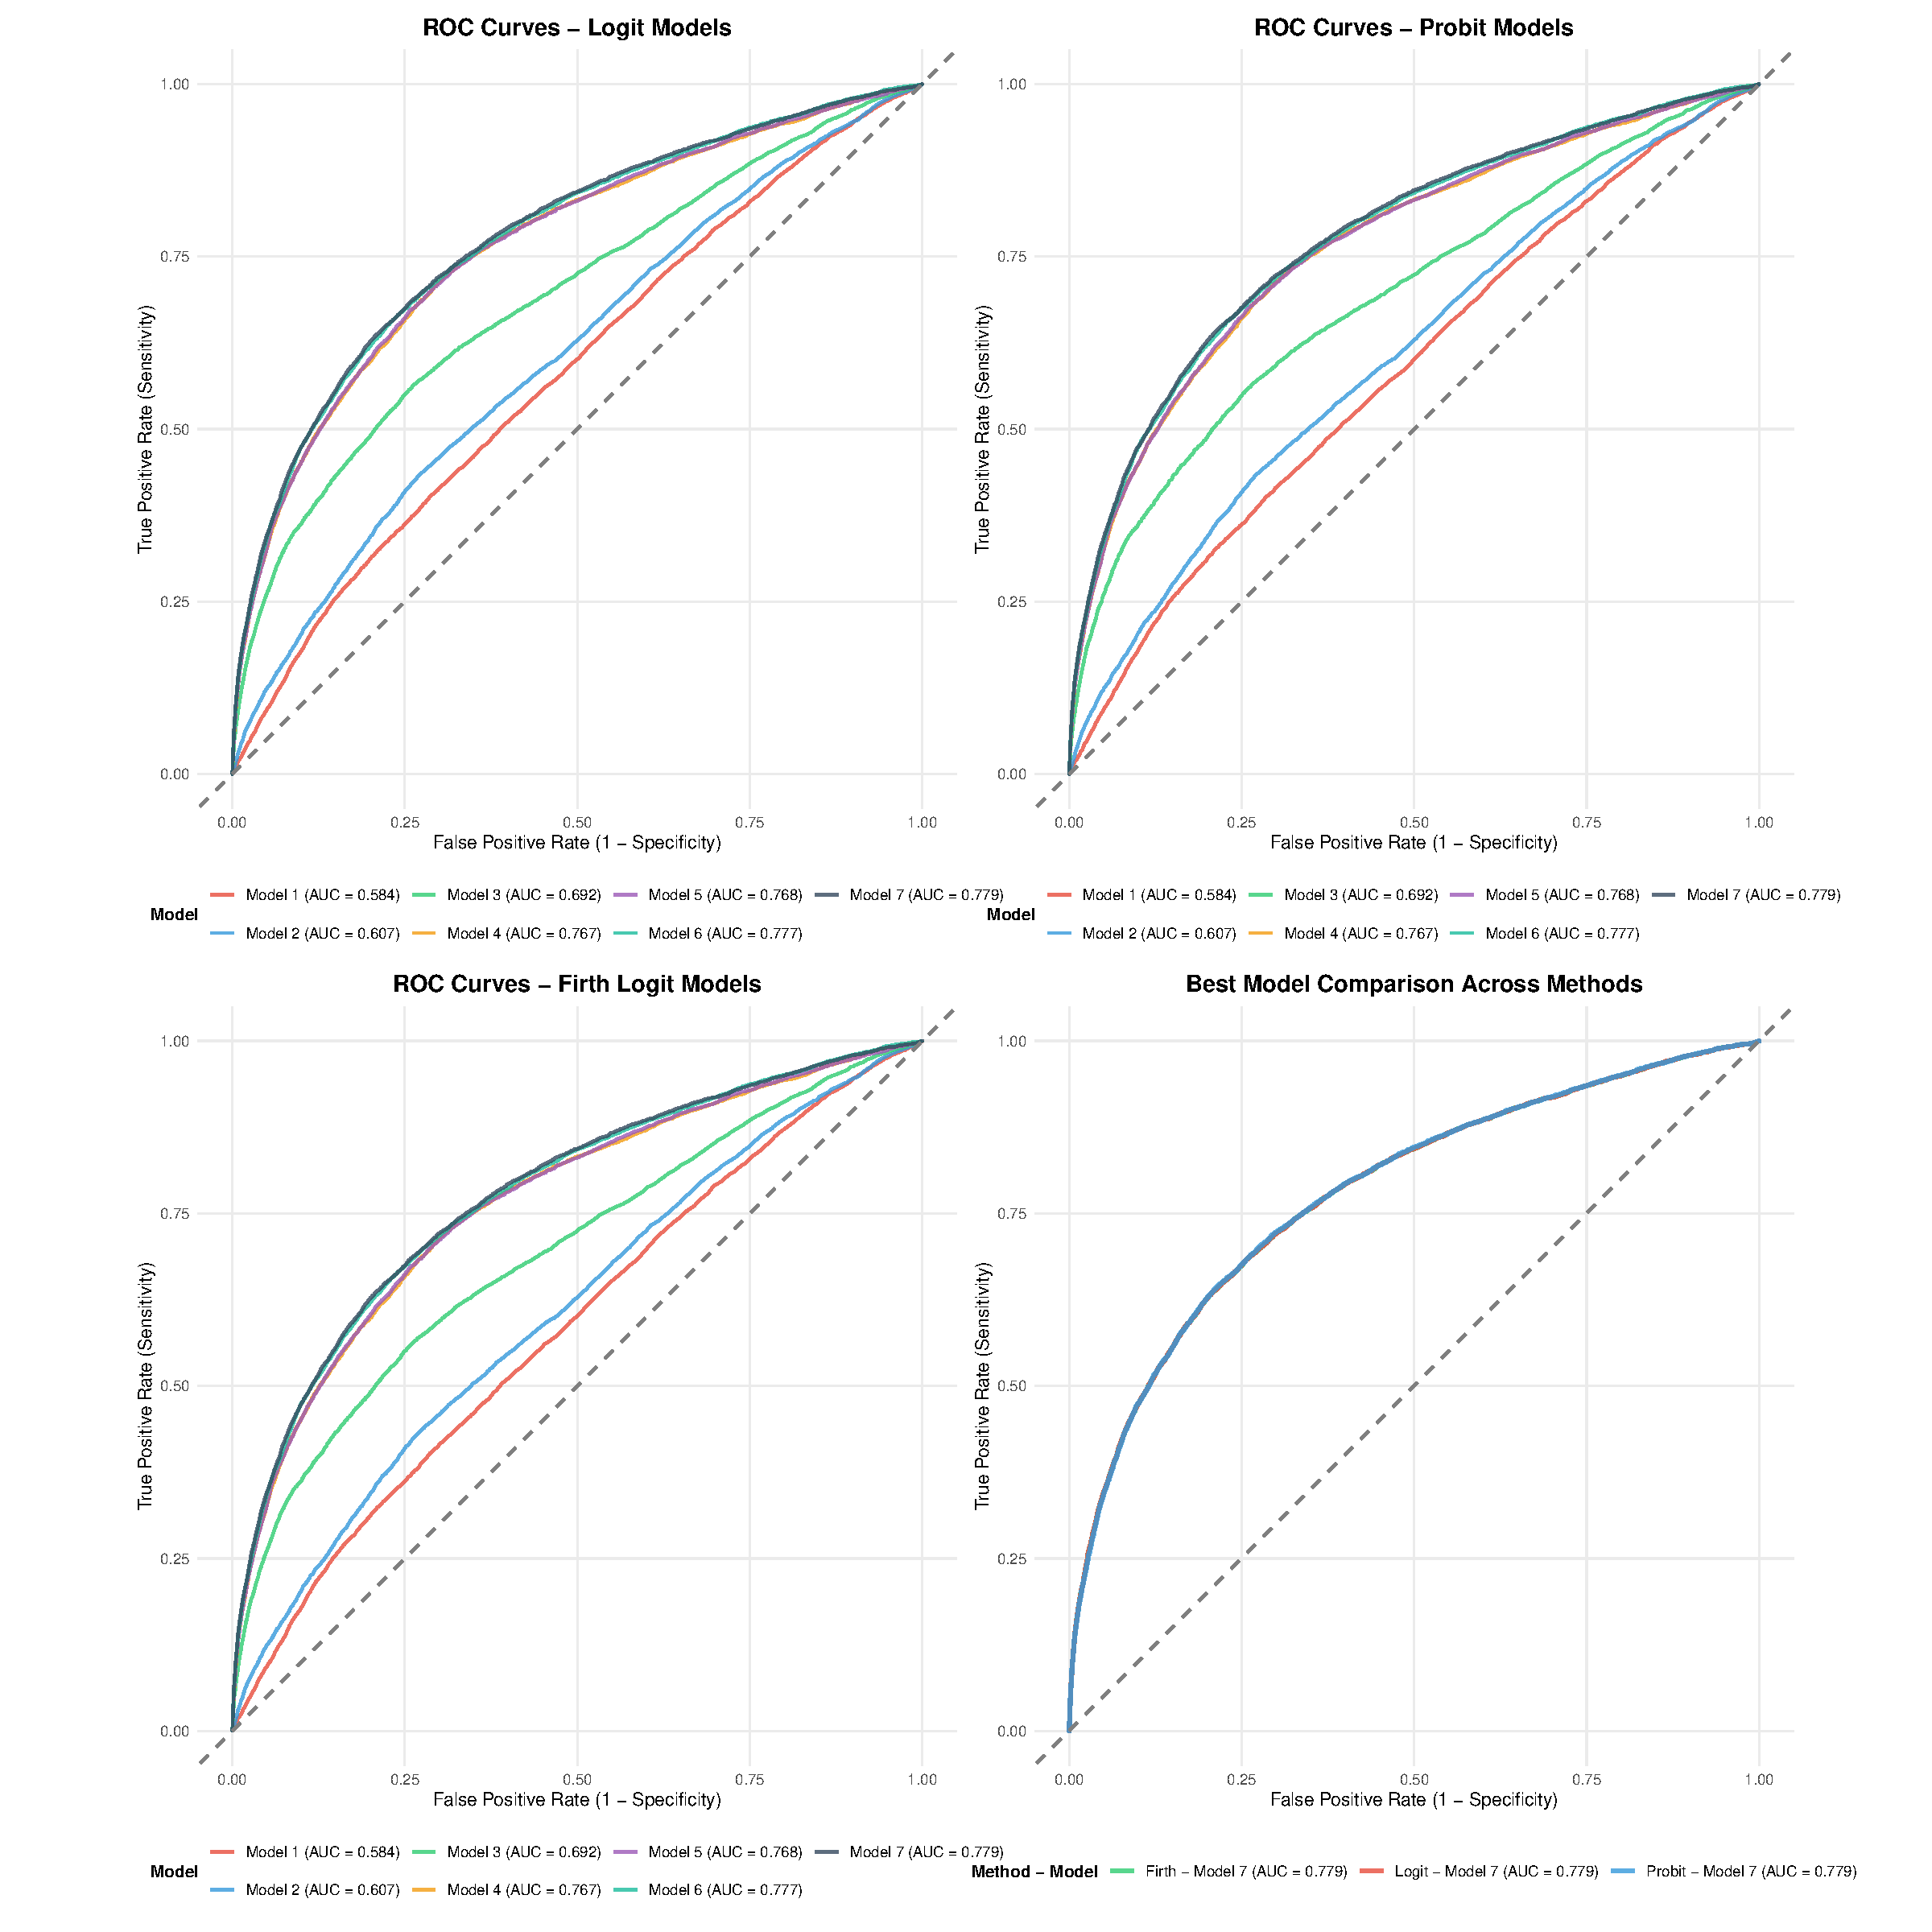
\includegraphics[keepaspectratio]{Trabajo_Amaru_Aguero_files/figure-pdf/unnamed-chunk-13-1.pdf}}

}

\caption{Curvas ROC (Característica Operativa del Receptor) que comparan
el rendimiento predictivo de siete modelos utilizando tres métodos de
estimación diferentes: regresión logística estándar (logit), regresión
probit y regresión logística penalizada de Firth. El cuarto panel
muestra una comparación del modelo con mejor rendimiento de cada método.
Cada curva muestra el equilibrio entre sensibilidad y especificidad con
los valores correspondientes del Área Bajo la Curva (AUC) para la
evaluación del modelo.}

\end{figure}%

\begin{figure}[H]

{\centering \pandocbounded{\includegraphics[keepaspectratio]{Trabajo_Amaru_Aguero_files/figure-pdf/unnamed-chunk-15-1.pdf}}

}

\caption{Diagnóstico para las variantes del Modelo 7 que muestra: (1)
Gráficos de calibración con la prueba de Hosmer-Lemeshow, (2) Residuos
de desviación versus valores ajustados y (3) Evaluación de
multicolinealidad utilizando el Factor de Inflación de Varianza
Generalizado (GVIF)}

\end{figure}%

\begin{figure}[H]

{\centering \pandocbounded{\includegraphics[keepaspectratio]{Trabajo_Amaru_Aguero_files/figure-pdf/unnamed-chunk-15-2.pdf}}

}

\caption{Diagnóstico para las variantes del Modelo 7 que muestra: (1)
Gráficos de calibración con la prueba de Hosmer-Lemeshow, (2) Residuos
de desviación versus valores ajustados y (3) Evaluación de
multicolinealidad utilizando el Factor de Inflación de Varianza
Generalizado (GVIF)}

\end{figure}%

\begin{figure}[H]

{\centering \pandocbounded{\includegraphics[keepaspectratio]{Trabajo_Amaru_Aguero_files/figure-pdf/unnamed-chunk-15-3.pdf}}

}

\caption{Diagnóstico para las variantes del Modelo 7 que muestra: (1)
Gráficos de calibración con la prueba de Hosmer-Lemeshow, (2) Residuos
de desviación versus valores ajustados y (3) Evaluación de
multicolinealidad utilizando el Factor de Inflación de Varianza
Generalizado (GVIF)}

\end{figure}%

\newpage

\begin{table}[H]
\centering
\caption{\label{tab:unnamed-chunk-16}Coeficientes Beta, Efecto Parcial en el Promedio (PEA) y Efecto Parcial Promedio (APE) con IC estándar para los modelos 7.}
\centering
\resizebox{\ifdim\width>\linewidth\linewidth\else\width\fi}{!}{
\fontsize{6.5}{8.5}\selectfont
\begin{tabular}[t]{>{\raggedright\arraybackslash}p{3cm}>{\centering\arraybackslash}p{2cm}>{\centering\arraybackslash}p{2cm}>{\centering\arraybackslash}p{2cm}>{\centering\arraybackslash}p{2cm}>{\centering\arraybackslash}p{2cm}>{\centering\arraybackslash}p{2cm}>{\centering\arraybackslash}p{2cm}>{\centering\arraybackslash}p{2cm}>{\centering\arraybackslash}p{2cm}}
\toprule
\multicolumn{1}{c}{ } & \multicolumn{3}{c}{Logit} & \multicolumn{3}{c}{Probit} & \multicolumn{3}{c}{Firth} \\
\cmidrule(l{3pt}r{3pt}){2-4} \cmidrule(l{3pt}r{3pt}){5-7} \cmidrule(l{3pt}r{3pt}){8-10}
Variable & Logit β & Logit PEA & Logit APE & Probit β & Probit PEA & Probit APE & Firth β & Firth PEA & Firth APE\\
\midrule
Substance: Other substances & 0.0257
(0.2865) & 0.0013
(0.0145)
[-0.0270, 0.0296] & 0.0016
(0.0175)
[-0.0327, 0.0358] & -0.0091
(0.1468) & -0.0010
(0.0164)
[-0.0332, 0.0312] & -0.0011
(0.0179)
[-0.0361, 0.0339] & 0.0520
(0.2836) & 0.0026
(0.0144)
[-0.0255, 0.0308] & 0.0032
(0.0173)
[-0.0308, 0.0372]\\
Substance: Cocaine & -0.0187
(0.0691) & -0.0009
(0.0035)
[-0.0078, 0.0059] & -0.0011
(0.0042)
[-0.0094, 0.0071] & -0.0125
(0.0352) & -0.0014
(0.0039)
[-0.0091, 0.0063] & -0.0015
(0.0043)
[-0.0099, 0.0069] & -0.0182
(0.0691) & -0.0009
(0.0035)
[-0.0078, 0.0059] & -0.0011
(0.0042)
[-0.0094, 0.0072]\\
Substance: Depressants & 0.4629***
(0.1124) & 0.0234†
(0.0057)
[0.0122, 0.0345] & 0.0283†
(0.0069)
[0.0148, 0.0417] & 0.2397***
(0.0595) & 0.0268†
(0.0067)
[0.0138, 0.0399] & 0.0292†
(0.0072)
[0.0150, 0.0433] & 0.4649***
(0.1122) & 0.0235†
(0.0057)
[0.0124, 0.0347] & 0.0284†
(0.0069)
[0.0150, 0.0419]\\
Substance: Marijuana & -0.0925
(0.1065) & -0.0047
(0.0054)
[-0.0152, 0.0059] & -0.0056
(0.0065)
[-0.0184, 0.0071] & -0.0525
(0.0528) & -0.0059
(0.0059)
[-0.0175, 0.0057] & -0.0064
(0.0064)
[-0.0190, 0.0062] & -0.0898
(0.1063) & -0.0045
(0.0054)
[-0.0151, 0.0060] & -0.0055
(0.0065)
[-0.0182, 0.0073]\\
Substance: Cocaine paste & 0.0425
(0.0565) & 0.0021
(0.0029)
[-0.0034, 0.0077] & 0.0026
(0.0035)
[-0.0042, 0.0094] & 0.0278
(0.0291) & 0.0031
(0.0033)
[-0.0033, 0.0095] & 0.0034
(0.0035)
[-0.0036, 0.0103] & 0.0423
(0.0565) & 0.0021
(0.0029)
[-0.0035, 0.0077] & 0.0026
(0.0035)
[-0.0042, 0.0094]\\
\addlinespace
Age & 0.0893***
(0.0078) & 0.0045†
(0.0004)
[0.0037, 0.0053] & 0.0055†
(0.0005)
[0.0045, 0.0064] & 0.0405***
(0.0037) & 0.0045†
(0.0004)
[0.0037, 0.0053] & 0.0049†
(0.0005)
[0.0040, 0.0058] & 0.0891***
(0.0078) & 0.0045†
(0.0004)
[0.0037, 0.0053] & 0.0055†
(0.0005)
[0.0045, 0.0064]\\
Age² & -0.0009***
(0.0001) & -0.0000†
(0.0000)
[-0.0001, -0.0000] & -0.0001†
(0.0000)
[-0.0001, -0.0000] & -0.0004***
(0.0000) & -0.0000†
(0.0000)
[-0.0001, -0.0000] & -0.0000†
(0.0000)
[-0.0001, -0.0000] & -0.0009***
(0.0001) & -0.0000†
(0.0000)
[-0.0001, -0.0000] & -0.0001†
(0.0000)
[-0.0001, -0.0000]\\
Sex: Male & -0.1045*
(0.0501) & -0.0053†
(0.0025)
[-0.0102, -0.0003] & -0.0064†
(0.0031)
[-0.0124, -0.0004] & -0.0583*
(0.0254) & -0.0065†
(0.0028)
[-0.0121, -0.0010] & -0.0071†
(0.0031)
[-0.0131, -0.0010] & -0.1049*
(0.0501) & -0.0053†
(0.0025)
[-0.0103, -0.0003] & -0.0064†
(0.0031)
[-0.0124, -0.0004]\\
Plan: Residential & 0.2791***
(0.0378) & 0.0141†
(0.0019)
[0.0103, 0.0178] & 0.0170†
(0.0023)
[0.0125, 0.0216] & 0.1548***
(0.0198) & 0.0173†
(0.0022)
[0.0130, 0.0217] & 0.0188†
(0.0024)
[0.0141, 0.0235] & 0.2790***
(0.0378) & 0.0141†
(0.0019)
[0.0104, 0.0179] & 0.0171†
(0.0023)
[0.0125, 0.0216]\\
N° previous mental hosp. & 0.4776***
(0.0114) & 0.0241†
(0.0006)
[0.0230, 0.0252] & 0.0292†
(0.0007)
[0.0278, 0.0305] & 0.2416***
(0.0062) & 0.0270†
(0.0007)
[0.0257, 0.0284] & 0.0294†
(0.0008)
[0.0279, 0.0309] & 0.4769***
(0.0114) & 0.0241†
(0.0006)
[0.0230, 0.0253] & 0.0292†
(0.0007)
[0.0278, 0.0305]\\
\addlinespace
Retreatments: 1 & 1.0479***
(0.0314) & 0.0529†
(0.0016)
[0.0498, 0.0560] & 0.0640†
(0.0019)
[0.0602, 0.0677] & 0.5120***
(0.0158) & 0.0573†
(0.0018)
[0.0538, 0.0608] & 0.0623†
(0.0019)
[0.0585, 0.0661] & 1.0473***
(0.0314) & 0.0530†
(0.0016)
[0.0499, 0.0561] & 0.0641†
(0.0019)
[0.0603, 0.0678]\\
Retreatments: 2 & 1.5968***
(0.0421) & 0.0806†
(0.0021)
[0.0764, 0.0847] & 0.0975†
(0.0026)
[0.0924, 0.1025] & 0.8077***
(0.0227) & 0.0904†
(0.0025)
[0.0854, 0.0954] & 0.0983†
(0.0028)
[0.0929, 0.1037] & 1.5958***
(0.0421) & 0.0808†
(0.0021)
[0.0766, 0.0849] & 0.0976†
(0.0026)
[0.0926, 0.1027]\\
Retreatments: 3+ & 2.2766***
(0.0437) & 0.1149†
(0.0022)
[0.1106, 0.1192] & 0.1390†
(0.0027)
[0.1337, 0.1442] & 1.2007***
(0.0247) & 0.1344†
(0.0028)
[0.1289, 0.1398] & 0.1461†
(0.0030)
[0.1402, 0.1520] & 2.2747***
(0.0437) & 0.1151†
(0.0022)
[0.1108, 0.1194] & 0.1391†
(0.0027)
[0.1339, 0.1444]\\
Education: Primary & -0.0665
(0.1856) & -0.0034
(0.0094)
[-0.0217, 0.0150] & -0.0041
(0.0113)
[-0.0263, 0.0181] & -0.0433
(0.0930) & -0.0048
(0.0104)
[-0.0252, 0.0155] & -0.0053
(0.0113)
[-0.0274, 0.0169] & -0.0779
(0.1846) & -0.0039
(0.0093)
[-0.0222, 0.0144] & -0.0048
(0.0113)
[-0.0269, 0.0174]\\
Education: Secondary & -0.0968
(0.1849) & -0.0049
(0.0093)
[-0.0232, 0.0134] & -0.0059
(0.0113)
[-0.0280, 0.0162] & -0.0604
(0.0926) & -0.0068
(0.0104)
[-0.0271, 0.0136] & -0.0073
(0.0113)
[-0.0294, 0.0147] & -0.1083
(0.1839) & -0.0055
(0.0093)
[-0.0237, 0.0128] & -0.0066
(0.0113)
[-0.0287, 0.0154]\\
\addlinespace
Education: University & 0.0488
(0.1890) & 0.0025
(0.0095)
[-0.0162, 0.0212] & 0.0030
(0.0115)
[-0.0196, 0.0256] & 0.0157
(0.0948) & 0.0018
(0.0106)
[-0.0190, 0.0225] & 0.0019
(0.0115)
[-0.0207, 0.0245] & 0.0378
(0.1880) & 0.0019
(0.0095)
[-0.0167, 0.0206] & 0.0023
(0.0115)
[-0.0202, 0.0249]\\
Education: Technical & 0.0163
(0.1880) & 0.0008
(0.0095)
[-0.0178, 0.0194] & 0.0010
(0.0115)
[-0.0215, 0.0235] & -0.0025
(0.0942) & -0.0003
(0.0105)
[-0.0209, 0.0204] & -0.0003
(0.0115)
[-0.0228, 0.0222] & 0.0052
(0.1870) & 0.0003
(0.0095)
[-0.0183, 0.0188] & 0.0003
(0.0114)
[-0.0221, 0.0227]\\
Marital: Married/Partnered & -0.1263**
(0.0444) & -0.0064†
(0.0022)
[-0.0108, -0.0020] & -0.0077†
(0.0027)
[-0.0130, -0.0024] & -0.0678**
(0.0224) & -0.0076†
(0.0025)
[-0.0125, -0.0027] & -0.0082†
(0.0027)
[-0.0136, -0.0029] & -0.1264**
(0.0444) & -0.0064†
(0.0022)
[-0.0108, -0.0020] & -0.0077†
(0.0027)
[-0.0131, -0.0024]\\
Marital: Other/No answer & 0.0293
(0.2742) & 0.0015
(0.0138)
[-0.0256, 0.0286] & 0.0018
(0.0167)
[-0.0310, 0.0346] & -0.0222
(0.1400) & -0.0025
(0.0157)
[-0.0332, 0.0282] & -0.0027
(0.0170)
[-0.0361, 0.0307] & 0.0536
(0.2715) & 0.0027
(0.0137)
[-0.0242, 0.0296] & 0.0033
(0.0166)
[-0.0293, 0.0358]\\
Marital: Single & 0.0157
(0.0436) & 0.0008
(0.0022)
[-0.0035, 0.0051] & 0.0010
(0.0027)
[-0.0043, 0.0062] & 0.0003
(0.0221) & 0.0000
(0.0025)
[-0.0048, 0.0049] & 0.0000
(0.0027)
[-0.0052, 0.0053] & 0.0154
(0.0436) & 0.0008
(0.0022)
[-0.0035, 0.0051] & 0.0009
(0.0027)
[-0.0043, 0.0062]\\
\addlinespace
Marital: Widowed & -0.1126
(0.1185) & -0.0057
(0.0060)
[-0.0174, 0.0060] & -0.0069
(0.0072)
[-0.0211, 0.0073] & -0.0654
(0.0601) & -0.0073
(0.0067)
[-0.0205, 0.0059] & -0.0080
(0.0073)
[-0.0223, 0.0064] & -0.1089
(0.1183) & -0.0055
(0.0060)
[-0.0172, 0.0062] & -0.0067
(0.0072)
[-0.0208, 0.0075]\\
Occupation: Studying & -0.1288
(0.1217) & -0.0065
(0.0061)
[-0.0185, 0.0055] & -0.0079
(0.0074)
[-0.0224, 0.0067] & -0.0742
(0.0595) & -0.0083
(0.0067)
[-0.0214, 0.0048] & -0.0090
(0.0072)
[-0.0232, 0.0052] & -0.1241
(0.1214) & -0.0063
(0.0061)
[-0.0183, 0.0058] & -0.0076
(0.0074)
[-0.0221, 0.0070]\\
Occupation: Other & -0.1189*
(0.0469) & -0.0060†
(0.0024)
[-0.0106, -0.0014] & -0.0073†
(0.0029)
[-0.0129, -0.0016] & -0.0643**
(0.0238) & -0.0072†
(0.0027)
[-0.0124, -0.0020] & -0.0078†
(0.0029)
[-0.0135, -0.0022] & -0.1184*
(0.0468) & -0.0060†
(0.0024)
[-0.0106, -0.0013] & -0.0072†
(0.0029)
[-0.0129, -0.0016]\\
Occupation: Retired/Pensioned & 0.3587***
(0.0916) & 0.0181†
(0.0046)
[0.0090, 0.0272] & 0.0219†
(0.0056)
[0.0109, 0.0329] & 0.1702***
(0.0482) & 0.0190†
(0.0054)
[0.0085, 0.0296] & 0.0207†
(0.0059)
[0.0092, 0.0322] & 0.3600***
(0.0915) & 0.0182†
(0.0046)
[0.0091, 0.0273] & 0.0220†
(0.0056)
[0.0111, 0.0330]\\
Occupation: Household tasks & -0.0922
(0.0553) & -0.0047
(0.0028)
[-0.0101, 0.0008] & -0.0056
(0.0034)
[-0.0122, 0.0010] & -0.0465
(0.0286) & -0.0052
(0.0032)
[-0.0115, 0.0011] & -0.0057
(0.0035)
[-0.0125, 0.0012] & -0.0918
(0.0552) & -0.0046
(0.0028)
[-0.0101, 0.0008] & -0.0056
(0.0034)
[-0.0122, 0.0010]\\
\addlinespace
Occupation: Working & -0.3805***
(0.0315) & -0.0192†
(0.0016)
[-0.0223, -0.0161] & -0.0232†
(0.0019)
[-0.0270, -0.0195] & -0.1860***
(0.0156) & -0.0208†
(0.0017)
[-0.0242, -0.0174] & -0.0226†
(0.0019)
[-0.0264, -0.0189] & -0.3803***
(0.0314) & -0.0192†
(0.0016)
[-0.0224, -0.0161] & -0.0233†
(0.0019)
[-0.0270, -0.0195]\\
Male × Other substances & 0.4652
(0.3503) & 0.0235
(0.0177)
[-0.0112, 0.0581] & 0.0284
(0.0214)
[-0.0135, 0.0703] & 0.2570
(0.1813) & 0.0288
(0.0203)
[-0.0110, 0.0685] & 0.0313
(0.0221)
[-0.0119, 0.0745] & 0.4498
(0.3475) & 0.0228
(0.0176)
[-0.0117, 0.0572] & 0.0275
(0.0213)
[-0.0141, 0.0692]\\
Male × Cocaine & -0.1646*
(0.0825) & -0.0083†
(0.0042)
[-0.0165, -0.0001] & -0.0100†
(0.0050)
[-0.0199, -0.0002] & -0.0784
(0.0413) & -0.0088
(0.0046)
[-0.0178, 0.0003] & -0.0095
(0.0050)
[-0.0194, 0.0003] & -0.1647*
(0.0824) & -0.0083†
(0.0042)
[-0.0165, -0.0002] & -0.0101†
(0.0050)
[-0.0200, -0.0002]\\
Male × Depressants & 0.1147
(0.1669) & 0.0058
(0.0084)
[-0.0107, 0.0223] & 0.0070
(0.0102)
[-0.0130, 0.0270] & 0.0611
(0.0883) & 0.0068
(0.0099)
[-0.0125, 0.0262] & 0.0074
(0.0107)
[-0.0136, 0.0285] & 0.1163
(0.1666) & 0.0059
(0.0084)
[-0.0106, 0.0224] & 0.0071
(0.0102)
[-0.0129, 0.0271]\\
Male × Marijuana & 0.1821
(0.1240) & 0.0092
(0.0063)
[-0.0031, 0.0215] & 0.0111
(0.0076)
[-0.0037, 0.0260] & 0.0955
(0.0613) & 0.0107
(0.0069)
[-0.0027, 0.0241] & 0.0116
(0.0075)
[-0.0030, 0.0262] & 0.1803
(0.1238) & 0.0091
(0.0063)
[-0.0032, 0.0214] & 0.0110
(0.0076)
[-0.0038, 0.0259]\\
\addlinespace
Male × Cocaine paste & -0.2568***
(0.0652) & -0.0130†
(0.0033)
[-0.0194, -0.0065] & -0.0157†
(0.0040)
[-0.0235, -0.0079] & -0.1255***
(0.0333) & -0.0140†
(0.0037)
[-0.0213, -0.0068] & -0.0153†
(0.0040)
[-0.0232, -0.0073] & -0.2565***
(0.0652) & -0.0130†
(0.0033)
[-0.0194, -0.0065] & -0.0157†
(0.0040)
[-0.0235, -0.0079]\\
\bottomrule
\multicolumn{10}{l}{\rule{0pt}{1em}\textit{Note: }}\\
\multicolumn{10}{l}{\rule{0pt}{1em}*** p < 0.001, ** p < 0.01, * p < 0.05 (significance for β coefficients)}\\
\multicolumn{10}{l}{\rule{0pt}{1em}† indicates 95\% CI does not contain zero (for marginal effects)}\\
\multicolumn{10}{l}{\rule{0pt}{1em}Standard errors in parentheses; 95\% CI in brackets}\\
\multicolumn{10}{l}{\rule{0pt}{1em}CI calculated using normal approximation with delta method standard errors}\\
\multicolumn{10}{l}{\rule{0pt}{1em}PEA = Partial Effect at the Average; APE = Average Partial Effect}\\
\multicolumn{10}{l}{\rule{0pt}{1em}Regional variables excluded from table}\\
\end{tabular}}
\end{table}

\begin{figure}[H]

{\centering \pandocbounded{
\includegraphics[keepaspectratio]{Trabajo_Amaru_Aguero_files/figure-pdf/unnamed-chunk-18-1.pdf}}

}

\caption{Efecto Parcial en el Promedio (PEA) y Efecto Parcial Promedio
(APE) para las interacciones entre sustancia principal y sexo en los
modelos 7. La figura muestra los efectos diferenciados por sexo para
cada tipo de sustancia comparada con alcohol, calculando la probabilidad
de hospitalización psiquiátrica para hombres y mujeres. Los intervalos
de confianza se calcularon usando el método delta con aproximación
normal.}

\end{figure}%

\newpage

\section{Discusión y Conclusiones}\label{discusiuxf3n-y-conclusiones}

\subsection{Marco teórico planteado y resultados
obtenidos}\label{marco-teuxf3rico-planteado-y-resultados-obtenidos}

El modelo teórico asumió un riesgo acumulativo en que la hospitalización
psiquiátrica depende de sustancias depresosaras del sistema nevioso
central y que interacciona con sexo. Otras variables importantes que
ajsutan el modelo y previene el sesgo por omisión es el historial
psiquiátrico: cada hospitalización mental previa aumentó
significativamente la probabilidad de otra hospitalización subsecuente.
Asimismo, los retratamientos mostraron un marcado efecto
dosis-respuesta: pacientes con ≥3 reingresos a tratamiento presentaron
una mayor APE de hospitalización que aquellos sin recaídas. El tipo de
tratamiento también fue significativo: la atención residencial se asoció
con mayor riesgo relativo a la ambulatoria, aunque parte de esta brecha
se redujo al controlar la mayor severidad de los casos derivados a
residencias.

En conjunto, estos hallazgos sustentan el modelo de riesgo acumulativo:
la combinación de vulnerabilidad psiquiátrica previa y alta severidad
adictiva incrementa sustancialmente el riesgo de descompensación mental,
concordando con evidencia internacional en patología dual que vincula la
comorbilidad adictiva-psiquiátrica a mayores tasas de hospitalización.

\subsection{Limitaciones del estudio}\label{limitaciones-del-estudio}

Este estudio observacional presenta varias limitaciones. Primero, la
naturaleza no experimental impide inferir causalidad sólida, dado que
pueden existir endogeneidades por variables omitidas; por ejemplo, el
efecto aparente del tratamiento residencial y el numeró de
retratamientos podría reflejar en parte la mayor gravedad clínica de sus
pacientes, pero que no se midió directamente. Segundo, el uso de
registros administrativos conlleva posibles sesgos de medición: las
recaídas podrían estar subreportadas (al considerar solo reingresos
formales) y solo se registran hospitalizaciones en el sistema de salud,
omitiendo episodios no atendidos o diagnósticos no consignados generando
una autoselciones de los casos más graves. Tercero, el modelo predictivo
mostró limitaciones de ajuste y poder explicativo: la prueba de
Hosmer-Lemeshow resultó significativa (falta de calibración) y la
capacidad discriminativa fue moderada (AUC \textasciitilde0.78), lo que
sugiere influencia de factores no observados. Cuarto, estos factores no
observados genera posibles sesgos de variables omitidas. Entre estas
variables están la severidad de la adicción, comorbilidades
psiquiátricas específicas, apoyo social y familiar, adherencia al
tratamiento, calidad del tratamiento, entre otras. Finalmente, para
afianzar las relaciones causales, se recomienda emplear diseños
cuasiexperimentales y datos longitudinales de seguimiento. Dichos
enfoques permitirían controlar mejor la endogeneidad, examinar la
secuencia temporal entre recaídas y hospitalizaciones, y aportar
evidencia más sólida para guiar intervenciones que reduzcan el riesgo de
hospitalización.

\newpage

\section{Repositorio GitHub}\label{repositorio-github}

Este código se replica autamáticamente con datos \textbf{simulados}
debido al tamaño de los datos originales. El código completo de este
análisis, incluyendo los modelos estadísticos, las visualizaciones y los
diagnósticos, está disponible en el siguiente
\href{https://github.com/AmaruSimonAgueroJimenez/Econometria-DCCS}{repositorio
GitHub}. De igual manera se puede acceder con el siguiente código QR.

\begin{center}
\pandocbounded{
\includegraphics[keepaspectratio]{Trabajo_Amaru_Aguero_files/figure-pdf/unnamed-chunk-20-1.pdf}}
\end{center}

El informe .pdf se encuentra en
\href{http://github.com/AmaruSimonAgueroJimenez/Econometria-DCCS/blob/main/docs/Trabajo_Amaru_Aguero.pdf}{esta
dirección}. De igual manera se puede acceder con el siguiente código QR.

\begin{center}
\pandocbounded{
\includegraphics[keepaspectratio]{Trabajo_Amaru_Aguero_files/figure-pdf/unnamed-chunk-21-1.pdf}}
\end{center}

\newpage

\section*{Referencias}\label{bibliography}
\addcontentsline{toc}{section}{Referencias}

\phantomsection\label{refs}
\begin{CSLReferences}{1}{0}
\bibitem[\citeproctext]{ref-Volkow2023}
1. Volkow, N. D., \& Blanco, C. (2023). Substance use disorders: a
comprehensive update of classification, epidemiology, neurobiology,
clinical aspects, treatment and prevention. \emph{World Psychiatry},
\emph{22}(2), 203-229. \url{https://doi.org/10.1002/wps.21073}

\bibitem[\citeproctext]{ref-Connery2020}
2. Connery, H. S., McHugh, R. K., Reilly, M., Shin, S., \& Greenfield,
S. F. (2020). Substance Use Disorders in Global Mental Health Delivery:
Epidemiology, Treatment Gap, and Implementation of Evidence-Based
Treatments. \emph{Harvard Review of Psychiatry}, \emph{28}(5), 316-327.
\url{https://doi.org/10.1097/HRP.0000000000000271}

\bibitem[\citeproctext]{ref-GomezSanchezLafuente2022}
3. Gómez-Sánchez-Lafuente, C., Guzman-Parra, J., Suarez-Perez, J.,
Bordallo-Aragon, A., Rodriguez-de-Fonseca, F., \& Mayoral-Cleries, F.
(2022). Trends in Psychiatric Hospitalizations of Patients With Dual
Diagnosis in Spain. \emph{Journal of Dual Diagnosis}, \emph{18}(2),
92-100. \url{https://doi.org/10.1080/15504263.2022.2053770}

\bibitem[\citeproctext]{ref-Saxena2011}
4. Saxena, S., Thornicroft, G., Knapp, J., \& Whiteford, M. (2007).
Resources for mental health: scarcity, inequity, and inefficiency.
\emph{World Psychiatry}, \emph{6}(1), 1-10.
\url{https://doi.org/10.1002/wps.21073}

\bibitem[\citeproctext]{ref-GomezSanchezLafuente2016}
5. Gómez-Sánchez-Lafuente, C., Guzman-Parra, J., Suarez-Perez, J.,
Mayoral-Cleries, F., \& Rodriguez-de-Fonseca, F. (2016). Dual Diagnosis
in Spain: Prevalence, Sociodemographic Profile, and Psychiatric
Comorbidity in a Sample of Patients Admitted to Psychiatric Inpatient
Units. \emph{Journal of Dual Diagnosis}, \emph{12}(3-4), 249-258.
\url{https://doi.org/10.1080/15504263.2016.1220207}

\bibitem[\citeproctext]{ref-Rojas2002}
6. Rojas, G., Gaete, M., Guajardo, M., Martínez, M., Martínez, M.,
Fritsch, R., \& Araya, R. (2002). Prevalencia de trastornos
psiquiátricos en pacientes hospitalizados en un hospital general.
\emph{Revista M{é}dica de Chile}, \emph{130}(6), 689-696.
\url{https://doi.org/10.4067/S0034-98872002000600008}

\bibitem[\citeproctext]{ref-cox1958regression}
7. Cox, D. R. (1958). The regression analysis of binary sequences (with
discussion). \emph{Journal of the Royal Statistical Society: Series B
(Methodological)}, \emph{20}(2), 215-242.
\url{https://doi.org/10.1111/j.2517-6161.1958.tb00292.x}

\bibitem[\citeproctext]{ref-bliss1934method}
8. Bliss, C. I. (1934). The method of probits. \emph{Science},
\emph{79}(2037), 38-39. \url{https://doi.org/10.1126/science.79.2037.38}

\bibitem[\citeproctext]{ref-firth1993bias}
9. Firth, D. (1993). Bias reduction of maximum likelihood estimates.
\emph{Biometrika}, \emph{80}(1), 27-38.
\url{https://doi.org/10.1093/biomet/80.1.27}

\bibitem[\citeproctext]{ref-neyman1933problem}
10. Neyman, J., \& Pearson, E. S. (1933). {IX}. {On} the problem of the
most efficient tests of statistical hypotheses. \emph{Philosophical
Transactions of the Royal Society of London. Series A},
\emph{231}(694-706), 289-337.
\url{https://doi.org/10.1098/rsta.1933.0009}

\bibitem[\citeproctext]{ref-akaike1973information}
11. Akaike, H. (1973). Information theory and an extension of the
maximum likelihood principle. En B. N. Petrov \& F. Csáki (Eds.),
\emph{Proceedings of the 2nd International Symposium on Information
Theory} (pp. 267-281). Akad{é}miai Kiad{ó}.

\bibitem[\citeproctext]{ref-hanley1982meaning}
12. Hanley, J. A., \& McNeil, B. J. (1982). The meaning and use of the
area under a receiver operating characteristic ({ROC}) curve.
\emph{Radiology}, \emph{143}(1), 29-36.
\url{https://doi.org/10.1148/radiology.143.1.7063747}

\bibitem[\citeproctext]{ref-delong1988comparing}
13. DeLong, E. R., DeLong, D. M., \& Clarke-Pearson, D. L. (1988).
\href{https://www.ncbi.nlm.nih.gov/pubmed/3203132}{Comparing the areas
under two or more correlated receiver operating characteristic curves: a
nonparametric approach}. \emph{Biometrics}, \emph{44}(3), 837-845.

\bibitem[\citeproctext]{ref-hosmer1980goodness}
14. Hosmer, D. W., \& Lemeshow, S. (1980). Goodness of fit tests for the
multiple logistic regression model. \emph{Communications in Statistics -
Theory and Methods}, \emph{9}(10), 1043-1069.
\url{https://doi.org/10.1080/03610928008827941}

\bibitem[\citeproctext]{ref-fox1992generalized}
15. Fox, J., \& Monette, G. (1992). Generalized collinearity
diagnostics. \emph{Journal of the American Statistical Association},
\emph{87}(417), 178-183.
\url{https://doi.org/10.1080/01621459.1992.10475190}

\end{CSLReferences}




\end{document}
